\documentclass[a4paper,leqno,twocolumn]{article}
% ==== Inputs and Usepackages ====

\usepackage{tablefootnote}
\usepackage{enumerate}
\usepackage{float}
\usepackage{url}
\usepackage{hyperref}
\usepackage{dsfont}
\usepackage{mathrsfs}
\usepackage{amsmath}
\usepackage{amssymb}
\usepackage{amsthm}
\usepackage{amsfonts}
\usepackage{mathtools}
%\usepackage{mathabx}
\usepackage{MnSymbol}
\usepackage{xfrac}
\usepackage{nicefrac}
\usepackage{geometry}
\usepackage{graphicx}
\usepackage{graphics}
\usepackage{latexsym}
\usepackage{setspace}
\usepackage{tikz-cd}
\usepackage{tikz}
 \usetikzlibrary{matrix}
 \usetikzlibrary{calc}
 \usetikzlibrary{circuits.ee.IEC}
\usepackage{circuitikz}

\usepackage{a4wide}
\usepackage{fancybox}
\usepackage{fancyhdr}
\usepackage[utf8]{inputenc}




% ==== Page Settings ====

\hoffset = -1.2 in
\voffset = -0.3 in
\textwidth = 590pt
\textheight = 770pt
\setlength{\headheight}{20pt}
\setlength{\headwidth}{590pt}
\marginparwidth = 0 pt
\topmargin = -0.75 in
\setlength{\parindent}{0cm}


% ==== Presettings for files ====

\pagestyle{fancy}


\cfoot{\thepage}
\lfoot{\href{mailto:szekerb@student.ethz.ch}{szekerb@student.ethz.ch}}
\rfoot{Balázs Szekér, \today}
\lhead{Physics \uproman{3} Summary}

% ==== General Commands ====

\newcommand{\sframebox}[1]{
        \framebox[500pt][l]{\parbox{490pt}{
            #1
        }
    }

}

\newcommand{\cframebox}[2]{
        \fbox{\parbox{#1pt}{
            #2
        }
    }
}









% ====== Maths ======


% ==== Formats ====
\newcommand{\boldline}[1]{\textbf{\underline{#1}}}
\newcommand{\uproman}[1]{\uppercase\expandafter{\romannumeral#1}}
\newcommand{\lowroman}[1]{\romannumeral#1\relax}
\newcommand{\fat}[1]{\textbf{#1}}
\newcommand{\Loesung}{\begin{center}\textbf{Lösung}\end{center}}

\newcommand{\Korollar}[1]{\textbf{Korollar} \vspace{1\baselineskip} #1}
\newcommand{\Beispiel}[1]{\textbf{Beispiel} \vspace{1\baselineskip} #1}
\newcommand{\Beweis}[1]{\textbf{Beweis} \vspace{1\baselineskip} #1}
\newcommand{\Proposition}[1]{\textbf{Proposition} \vspace{1\baselineskip} #1}
\newcommand{\Satz}[1]{\textbf{Satz} \vspace{1\baselineskip} #1}
\newcommand{\Definition}[1]{\textbf{Definition} \vspace{1\baselineskip} #1}
\newcommand{\Lemma}[1]{\textbf{Lemma}\vspace{1\baselineskip} #1}
\newcommand{\Bemerkung}[1]{\textbf{Bemerkung} \vspace{1\baselineskip} #1}
\newcommand{\Theorem}[1]{\textbf{Theorem} \vspace{1\baselineskip} #1}




% ==== mathsymbols ====
\newcommand{\Q}{\mathbb{Q}}
\newcommand{\R}{\mathbb{R}}
\newcommand{\N}{\mathbb{N}}
\newcommand{\Z}{\mathbb{Z}}
\newcommand{\C}{\mathbb{C}}
\newcommand{\K}{\mathbb{K}}
\newcommand{\eS}{\mathbb{S}}
\newcommand{\X}{$X$ }
\newcommand{\Y}{$Y$ }
\newcommand{\x}{$x$ }
\newcommand{\y}{$y$ }
\newcommand{\B}{\mathcal{B}}
\newcommand{\A}{\mathcal{A}}
\renewcommand{\S}{\mathcal{S}}
\renewcommand{\P}{\mathcal{P}}



% ==== math operators ====
\newcommand{\klammer}[1]{\left( #1 \right)} 
\newcommand{\eckigeklammer}[1]{\left[ #1 \right]}
\newcommand{\geschwungeneklammer}[1]{\left\{ #1 \right\}}
\newcommand{\floor}[1]{\left\lfloor #1 \right\rfloor}
\newcommand{\ceil}[1]{\left\lceil #1 \right\rceil}
\newcommand{\scalprod}[2]{\left\langle #1 , #2 \right\rangle}
\newcommand{\abs}[1]{\left\vert #1 \right\vert} 
\newcommand{\Norm}[1]{\left\vert\left\vert #1 \right\vert\right\vert}
\newcommand{\intab}{\int_a^b}
\newcommand{\intii}{\int_{-\infty}^\infty} 
\newcommand{\cint}[2]{\int_{#1}^{#2}}
\newcommand{\csum}[2]{\sum_{#1}^{#2}}
\newcommand{\limes}[1]{\lim\limits_{#1}}
\newcommand{\limessup}[1]{\limsup\limits_{#1}}
\newcommand{\limesinf}[1]{\liminf\limits_{#1}}
\newcommand{\limesninf}{\limes{n \rightarrow \infty}}
\newcommand{\limsupninf}{\limessup{n \rightarrow \infty}}
\newcommand{\liminfninf}{\limesinf{n \rightarrow \infty}}
\newcommand{\standardNorm}{\Norm{ \ \cdot \ }}
\newcommand{\einsNorm}{\Norm{ \ \cdot \ }_1}
\newcommand{\zweiNorm}{\Norm{ \ \cdot \ }_2}
\newcommand{\Hom}{\text{Hom}}
\newcommand{\Mat}{\text{Mat}}
\newcommand{\grad}{\text{grad}}
\newcommand{\vol}{\text{vol}}
\newcommand{\supp}{\text{supp}}
\newcommand{\rot}{\text{rot}}
\renewcommand{\div}{\text{div}}



% ==== Analysis ====
\newcommand{\supremum}{\text{sup}}
\newcommand{\infimum}{\text{inf}}
\newcommand{\maximum}{\text{max}}
\newcommand{\minimum}{\text{min}}

\newcommand{\xinX}{$x \in X$ }
\newcommand{\yinY}{$y \in Y$ }
\newcommand{\xyinX}{$x,y \in X$ }
\newcommand{\yinX}{$y \in X$ }
\newcommand{\xinR}{$x \in \R$ }
\newcommand{\xyinR}{$x,y \in \R$ }
\newcommand{\zinC}{$z \in \C$ }
\newcommand{\ninN}{$n \in \N$ }
\newcommand{\NinN}{$N \in \N$}
\newcommand{\angeordneterK}{$(K,\leq)$ }
\newcommand{\xFolge}{(x_n)_{n=0}^{\infty}}
\newcommand{\yFolge}{(y_n)_{n=0}^{\infty}}
\newcommand{\zFolge}{(z_n)_{n=0}^{\infty}}
\newcommand{\aFolge}{(a_n)_{n=0}^{\infty}}
\newcommand{\fFolge}{(f_n)_{n=0}^{\infty}}

\newcommand{\XsubR}{$X \subset \R$ }
\newcommand{\XsubeqR}{$X \subseteq \R$ }

\newcommand{\XFam}{\mathcal{X}}
\newcommand{\PFam}{\mathcal{P}}

\newcommand{\offenesintervall}[2]{$\left( #1 , #2 \right)$ }
\newcommand{\abgeschlossenesintervall}[2]{$\left( #1 , #2 \right)$ }

\newcommand{\XTopRaum}{(X,\tau)}


% ==== Lineare Algebra ====
\newcommand{\vinV}{$v \in V$ }
\newcommand{\uinU}{$u \in U$ }
\newcommand{\winW}{$w \in W$ }
\newcommand{\vwinV}{$v,w \in V$ }

\newcommand{\BasisV}{v_1 , \dots , v_n}
\newcommand{\BasisU}{u_1 , \dots , u_n}
\newcommand{\BasisW}{w_1 , \dots , w_n}

\newcommand{\transpose}[1]{#1^t}
\newcommand{\inverse}[1]{#1^{-1}}
\newcommand{\ddvec}[3]{\left( #1,#2,#3 \right)}
\newcommand{\tdvec}[2]{\left( #1 , #2 \right)}

\newcommand{\Edrei}{\begin{pmatrix}
    1 & 0 & 0 \\
    0 & 1 & 0 \\
    0 & 0 & 1
\end{pmatrix}}

\newcommand{\id}{\text{id}}
\newcommand{\GL}{\text{GL}}
\newcommand{\End}{\text{End}}
\renewcommand{\Im}{\text{Im}}
\renewcommand{\Re}{\text{Re}}
\renewcommand{\ker}{\text{Ker}}
\newcommand{\rang}{\text{rang}}
\newcommand{\ad}{\text{ad}}
\newcommand{\Eig}{\text{Eig}}
\newcommand{\Bil}{\text{Bil}}
\newcommand{\sign}{\text{sign}}
\newcommand{\tr}{\text{tr}}



% ====== Physics ======

% ==== Physicssymbols ====
\newcommand{\epsilonnull}{\epsilon_0}
\newcommand{\munull}{\mu_0}
\newcommand{\rn}{r_0}
\newcommand{\Rn}{R_0}
\newcommand{\rhonull}{\rho_0}
\newcommand{\Rhonull}{\varrho_0}


% ==== Notation ====
\newcommand{\Etot}{E_{\text{Tot}}}
\newcommand{\Wtot}{W_{\text{Tot}}}
\newcommand{\Ftot}{F_{\text{Tot}}}
\newcommand{\vtot}{v_{\text{Tot}}}
\newcommand{\atot}{a_{\text{Tot}}}
\newcommand{\mtot}{m_{\text{Tot}}}
\newcommand{\Mtot}{M_{\text{Tot}}}

\newcommand{\Ekin}{E_{\text{Kin}}}
\newcommand{\Epot}{E_{\text{Pot}}}
\newcommand{\Edef}{E_{\text{Def}}}

\newcommand{\Fg}{F_g}
\newcommand{\FN}{F_N}
\newcommand{\Fz}{F_z}
\newcommand{\FC}{F_C}

\newcommand{\xn}{x_0}
\newcommand{\xN}{x_n}
\newcommand{\vn}{v_0}
\newcommand{\vN}{v_n}
\newcommand{\an}{a_0}
\newcommand{\aN}{a_n}

\newcommand{\dt}{\Delta t}
\newcommand{\dx}{\Delta x}
\newcommand{\dv}{\Delta v}
\newcommand{\da}{\Delta a}
\newcommand{\dE}{\Delta E}
\newcommand{\dW}{\Delta W}
\newcommand{\dF}{\Delta F}


% ==== Relativity ====
\newcommand{\relsqrt}{\sqrt{1-\frac{v^2}{c^2}}}
\newcommand{\relgamma}{\frac{1}{\relsqrt}}


% ==== Constants ====
\newcommand{\g}{9.81}





\renewcommand*{\figurename}{Abb.}
\renewcommand{\epsilon}{\varepsilon}
\clubpenalty = 10000
\widowpenalty = 10000

\theoremstyle{definition}
\newtheorem*{theorem}{Theorem}
\newtheorem*{definition}{Definition}
\newtheorem*{lemma}{Lemma}
\newtheorem*{proposition}{Proposition}
\newtheorem*{beispiel}{Beispiel}
\newtheorem*{korollar}{Korollar}
\newtheorem*{bemerkung}{Bemerkung}
\newtheorem*{beweis}{Beweis}

\setcounter{section}{-1}

\begin{document}

\section{Grundlagen}

\begin{align*}
    \frac{\partial x}{\partial y} \Big|_z
    &= \klammer{\frac{\partial y}{\partial x} \Big|_z}^{-1}
    \hspace{5pt} , \hspace{5pt}
    - 1 = \frac{\partial x}{\partial y} \Big|_z \frac{\partial y}{\partial z} \Big|_x \frac{\partial z}{\partial x} \Big|_y
    \hspace{5pt} , \hspace{5pt}
    \frac{\partial x}{\partial w} \Big|_z = \frac{\partial x}{\partial y} \Big|_z \frac{\partial y}{\partial w} \Big|_z
    \\
    \frac{\partial x}{\partial z} \Big|_w &= \frac{\partial x}{\partial y} \Big|_w \frac{\partial y}{\partial z} \Big|_w
    \hspace{5pt} , \hspace{5pt}
    \frac{\partial x}{\partial y} \Big|_z = \frac{\partial x}{\partial y} \Big|_w + \frac{\partial x}{\partial w} \Big|_y \frac{\partial w}{\partial y} \Big|_z
\end{align*}

\begin{enumerate}[]
    \item \underline{allgemein}: $dU = \delta Q + \delta W$
    \item \underline{adiabatisch}: $\delta Q = 0 \ \Rightarrow \ dU = \delta W = - p dV$
    \item \underline{isotherm}: $dT = 0 \ \Rightarrow \ dU = 0 \ \Rightarrow \ \delta Q = - \delta W = p dV$
    \item \underline{isochor}: $d V = 0 \ \Rightarrow \ dU = \delta Q = C_V dT$
    \item \underline{isobar}: $dp = 0 \ \Rightarrow \ \delta Q = C_p dT$ 
\end{enumerate}

\paragraph{Adiabatengleichung}
Für ideale Gase gilt bei einem adiabatischen Prozess:
($\gamma - 1 = \frac{R}{c_v}$, $\gamma = \frac{c_p}{c_v}$, $\alpha = 1 - \gamma^{-1} > 0$,
$\alpha = \frac{\kappa - 1}{\kappa}$)
\begin{align*}
    T V^{\gamma - 1} = \text{const}
    \hspace{5pt} , \hspace{5pt}
    T p^{-\alpha} = \text{const}
    \hspace{5pt} , \hspace{5pt}
    p V^\kappa = \text{const}
    \hspace{5pt} , \hspace{5pt}
    T^\kappa p^{(1-\kappa)} = \text{const}
\end{align*}



\section{Hauptsätze der Thermodynamik}

\subsection{Thermodynamische Systeme und ihr Gleichgewicht}

\paragraph{Zustandsvariablen}
Grössen die bestimmbar sind. Bsp: V,p,T

\paragraph{Thermodynamisches System}
Wir bezeichnen mit $S$ ein thermodynamisches System. Eine Abfolge von
Zuständen eines Systems wird mit $\geschwungeneklammer{\sigma_i}_{i=1,\dots,n}$
bezeichnet.

\subsection{Grundbegriffe: System, Prozesse, Zustände, Arbeit}

\subsubsection{Systeme}
Wir nennen die Menge von Systemen $\S$. Jedes System $S \in \S$ ist
aufgebaut aus atomischen (thermodynamischen) Systemen, welche selbts eine
nicht-leere Untermenge $\A \subset \S$ bilden. Atomische Systeme sind in
einem thermodynamischen Sinne unteilbar.

\begin{definition}[Zusammensetzen von Systemen]
    Für eine endliche Anzahl thermodynamischer Systeme $S_1,\dots,S_n \in \S$
    ist das System $S$, welche aus diesen zusammengesetzt ist, definiert
    durch
    \begin{align*}
        \text{Atom}(S) := \text{Atom}(S_1) \cup \dotsb \cup \text{Atom}(S_n)
    \end{align*}
    und wir schreiben $S = S_1 \vee \dotsb \vee S_n$.
\end{definition}

\begin{definition}[Schnitt und disjunkte Systeme]
    Für zwei Systeme $S_1,S_2 \in \S$ ist ihr Schnitt $S_1 \wedge S_2$
    definiert durch
    \begin{align*}
        \text{Atom}(S_1 \wedge S_2) := \text{Atom}(S_1) \cap \text{Atom}(S_2)
    \end{align*}
    Wenn die Schnittmenge $\text{Atom}(S_1) \cap \text{Atom}(S_2)$ leer ist, schreiben
    wir $S_1 \wedge S_2 = \emptyset$ und nennen die Systeme disjunkt.
\end{definition}

\begin{definition}[Untersysteme]
    Für ein System $S \in \S$ ist die Menge seiner Untersysteme definiert durch
    \begin{align*}
        \text{Sub}(S) := \geschwungeneklammer{S' \in \S \ | \ S' \vee S = S}
    \end{align*}
    Für jedes echte Untersystem $S' \in \text{Sub}(S)$, $S' \neq S$, gibt es
    ein eindeutiges disjunktes Komplement $S'' \in \S$, so dass $S' \vee S'' = S$.
\end{definition}


\subsubsection{Prozesse}
Es gibt eine nicht-leere Menge $\P$ von (thermodynamischen) Prozessen.
Jeder Prozess definiert den Anfangs- und Endzustand auf einem atomischen
System $A \in \A$, auf dem er wirkt. Für jedes $A \in \A$ gibt es Funktionen
$\floor{.}_A : \P \rightarrow \Sigma_A$ und $\ceil{.}_A : \P \rightarrow
\Sigma_A$ die einen thermodynamischen Prozess auf den Anfangs- und Endzustand
auf dem System $A$ abbildet und wir sagen, dass das System $A$ in $p$
involviert ist (auch: $p$ wirkt auf $A$). Der Raum $\Sigma_A$ heisst
Zustandsraum von $A$. Für $A_1 \neq A_2$ gilt $\Sigma_{A_1} \cap \Sigma_{A_2}
= \emptyset$. Wir fordern, dass $\forall \ p \in \P$ die Funktionen
$\floor{p}_A$ und $\ceil{p}_A$ für mindestens eines und höchstens endlich
viele $A \in \A$ definiert sind.

\begin{definition}[Zustände allgemeiner Systeme]
    Sei $S = A_1 \vee \dotsb \vee A_n$. Für einen thermodynamischen
    Prozess $p \in \P$ ist der Anfangszustand auf $S$ definiert durch
    \begin{align*}
        \floor{.}_S : \P &\rightarrow \Sigma_S
        \\
        p &\mapsto \floor{p}_S := \klammer{\floor{p}_{A_1},\dots,\floor{p}_{A_n}}
    \end{align*}
    und analog für den Endzustand mittels $\ceil{.}$. Für diskunkte Systeme
    $S_1 , S_2 \in \S$ mit Zuständen $\sigma_1 \in \Sigma_{S_1}$ und $\sigma_2
    \in \Sigma_{S_2}$ verwenden wir die Schreibweise $(\sigma_1 , \sigma_2) =:
    \sigma_1 \vee \sigma_2 = \sigma_2 \vee \sigma_1 \in \Sigma_{S_1} \vee \Sigma_{S_2}$.
\end{definition}

\begin{definition}[Zustandsgrösse]
    Eine Zustandsgrösse eines Systems $S$ (auch Zustandsvariable oder
    Zusatndsfunktion) ist eine Funktion von $\Sigma_S$ in einen Zielraum
    $\mathcal{Z}$, $Z: \Sigma_S \Rightarrow \mathcal{Z}$. Der Zielraum ist
    typischerweise $\mathcal{Z} = \R^n$, meistens sogar $n=1$. Wir schreiben
    $\Delta Z(p) := Z(\ceil{p}_S) - Z(\floor{p}_S)$ für die Änderung einer
    Zustandsgrösse unter einem Prozess $p \in \P$.
\end{definition}

\paragraph{Verknüpfung von Prozessen}
Die Konkatenierung (Hintereinanderausführung) der Prozesse $p,p' \in \P$
zu $p' \circ p$ ist immer mödlich, sobald $\forall A \in \A$ entweder die
Gleichung $\ceil{p}_A = \floor{p'}_A$ gilt, oder mindestens eine der
Seiten undefiniert ist. Ausserdem soll $\circ$ kommutativ sein, für
Prozesse, deren Zustandsänderungen auf disjunkten Untermengen von $\A$
definiert sind. Die Menge der Prozesse $\P$ soll abgeschlossen sein unter
$\circ$. Auf einem beliebigen atomischen System $A \in \A$ gilt:
\begin{align*}
    \floor{p' \circ p}_A = \begin{cases}
        \floor{p}_A \hspace{10pt} &\text{falls } \floor{p}_A \text{ def.}
        \\
        \floor{p'}_A \hspace{10pt} &\text{falls } \floor{p}_A \text{ undef. aber } \floor{p'}_A \text{ def.}
        \\
        \text{undef.} \hspace{10pt} &\text{falls beide } \floor{p}_A \text{ und } \floor{p'}_A \text{ undef.}
    \end{cases}
\end{align*}
sowie Analoges für den Endzustand. Falls $p$ und $p'$ auf disjunkten Systemen
agieren, schreiben wir $p \vee p'$ anstatt $p \circ p' = p' \circ p$.


\paragraph{Arbeitsfunktion}
Für jedes atomisches System $A \in \A$ gibt es eine Arbeitsfunktion
$W_A : \P \rightarrow \R$, welche einem beliebigen Prozess die Arbeit zuordnet,
die während dem Prozess in $A$ investiert wurde. Falls $A$ nicht in $p$
involviert ist, soll $W_A (p) = 0$ gelten. Weiter gilt für $p,p' \in \P$
so dass $p' \circ p$ wohldefiniert ist:
\begin{align*}
    W_A (p' \circ p) = W_A (p) + W_A (p') \ \ \forall A \in \A
\end{align*}
\underline{Konvention}: $W_A$ ist positiv, falls Arbeit aufgewendet werden
muss, also in das System investiert wird. Wenn das System selbst Arbeit
leistet, ist $W_A$ demnach negativ.

\begin{definition}[Arbeitskosten für allgemeine Systeme]
    Für ein beliebiges System $S \in \S$ definieren wir die Arbeitsfunktion
    $W_S : \P \rightarrow \R$ als die Summe der Arbeitsfunktionen der
    Atomischen Untersysteme:
    \begin{align*}
        W_S := \sum_{A \in \text{Atom}(S)} W_A
    \end{align*}
    Für $S_1,S_2 \in \S$ mit $S_1 \wedge S_2 = \emptyset$ und $\forall \ 
    p \in \P$ gilt:
    \begin{align*}
        W_{S_1 \vee S_2} (p) = W_{S_1} (p) + W_{S_2} (p)
    \end{align*}
\end{definition}

\begin{definition}[Identitätsprozess]
    Ein Identitätsprozess soll immer, also für jedes beliebige System in
    jedem beliebigen Anfangszustand, möglich sein. Es ist der Prozess, bei
    dem wir einfach nichts tun. Für so einen Prozess $\id_S^\sigma$ auf $S$
    im Zustand $\sigma$ gilt dann $\floor{\id_S^\sigma}_S = \sigma =
    \ceil{\id_S^\sigma}_S$. Die Arbeitskosten sind Null.
\end{definition}


\subsection{Arbeitsprozesse und der 1. Hauptsatz}

\begin{definition}[Arbeitsprozesse auf $S$]
    Für ein System $S \in \S$ ist $\P_S$ die Menge aller Prozesse, die
    genau auf $S$ wirkt. Wir nennen diese Arbeitsprozesse auf $S$.
    \begin{align*}
        \P_S := \geschwungeneklammer{p \in \P \ | \ \floor{p}_{S'} \text{ ist def. genau für $S' \in \text{Sub}(S)$}}
    \end{align*}
    Arbeitsprozesse auf $S$ sind also Prozesse, für welche $S$ das "grösste"
    System ist, auf dem sie wirken.
\end{definition}

\begin{definition}[Zyklische und Identitätsprozesse]
    Ein thermodynamischer Prozess $p \in \P$ heisst zyklisch auf $S \in \S$,
    falls $\floor{p}_S = \ceil{p}_S$. Er heisst Identitätsprozess, wenn er
    ein Arbeitsprozess $p \in \P_S$ auf $S$ ist. Für Identitätsprozesse auf
    $S$, die den Zusatand $\sigma$ invariant lassen, benutzen wir die Notation
    $p = \id_S^\sigma = \id_S$. 
\end{definition}

\begin{definition}[Reversibler Arbeitsprozess]
    Ein Arbeitsprozess $p \in \P_S$ auf einem System $S$ heisst reversibel,
    falls es einen Arbeitsprozess $p^{rev} \in \P_S$ gibt, so dass
    $p^{rev} \circ p$ ein Identitätsprozess ist. Insbesondere ist dann
    $p^{rev} \circ p$ definiert.
\end{definition}

\paragraph{1. Hauptsatz}
Für jedes System $S \in \S$ gilt:
\begin{enumerate}[(i)]
    \item Zu jedem Paar von Zuständen $\sigma_1 , \sigma_2 \in \Sigma_S$
        gibt es einen Arbeitsprozess $p \in \P_S$ auf diesem System, so dass
        $\floor{p}_S = \sigma_1$ und $\ceil{p}_S = \sigma_2$ oder es gibt
        $p' \in \P_S$ so dass $\floor{p'}_S = \sigma_2$ und $\ceil{p'}_S =
        \sigma_1$.
    \item Die Arbeitskosten eines Prozesses $p \in \P_S$ mit Anfangszustand
        $\sigma_1$ und Endzustand $\sigma_2$ hängt nur vom geordneten Paar
        $(\sigma_1,\sigma_2)$ ab und nicht vom Prozess $p$. D.h. falls es
        einen anderen Prozess $p'' \in \P_S$ gibt, welcher die gleichen
        Zustände in der gleichen Richtung ineinander überführt, so gilt
        $W_S (p'') = W_S (p)$.
\end{enumerate}

\begin{bemerkung}
    Es gilt $W_S(\id_S^\sigma) = 0$. Weiter gilt für jeden reversiblen
    Arbeitsprozess $p \in \P_S$ mit Umkehrprozess $p^{rev} \in \P_S$:
    \begin{align*}
        W_S (p^{rev}) = - W_S(p)
    \end{align*}
\end{bemerkung}

\begin{definition}[Innere Energie]
    Die (innere) Energie eines Systems $S$ im Zustand $\sigma \in \Sigma_S$
    ist definiert als
    \begin{align*}
        U_S (\sigma) &:= W_S + U_0
        \hspace{10pt} , \hspace{10pt}
        \text{falls } p \in \P_S \ \sigma_0 \text{ in } \sigma \text{ überführt}
        \\
        U_S (\sigma) &:= - W_S (p') + U_0
        \hspace{10pt} , \hspace{10pt}
        \text{falls } p' \in \P_S \ \sigma \text{ in } \sigma_0 \text{ überführt}
    \end{align*}
    Wobei $\sigma_0 \in \Sigma_S$ ein beliebiger aber fixer Referenzzustand ist
    und $U_0 \in \R$ eine willkürkliche aber fixe Energiekonstante.
\end{definition}


\subsection{Wärme}

\begin{definition}[Wärme]
    Sei $p \in \P$ ein beliebiger Prozess. Dann ist die $S$ zufliessende
    Wärme definiert als
    \begin{align*}
        Q_S (p) := \Delta U_S (p) - W_S (p)
        \hspace{10pt} , \hspace{10pt}
        \Delta U_S (p) := \sum_{\stackrel{A \in \text{Atom}(S)}{A \text{ inv. in } p}} \Delta U_A (p)
    \end{align*}
    Wärme ist also die Energie, die zwischen Systemen ausgetauscht wird
    und dadurch die innere Energie der betroffenen Systeme verändert, welche
    nicht Arbeit ist.
\end{definition}

\paragraph{Notation} $W_S := W_S(p)$ und $Q_S = Q_S(p)$

\begin{definition}[Quasistatischer Prozess]
    Ein quasistatischer Arbeitsprozess auf einem System $S \in \S$ ist eine
    zweiparametrige Familie von Arbeitsprozessen
    $\geschwungeneklammer{p(\lambda,\lambda')}_{\lambda,\lambda'} \subset
    \P_S$ mit $\lambda,\lambda' \in [0,1]$ und $\lambda \leq \lambda'$
    und den Eigenschaften:
    \begin{enumerate}[(i)]
        \item Für $\lambda \leq \lambda' \leq \lambda'' \in [0,1]$ gilt
            $p(\lambda',\lambda'') \circ p(\lambda,\lambda') = p(\lambda,\lambda'')$
            $\Rightarrow \ceil{p(\lambda,\lambda')}_S = \floor{p(\lambda',\lambda'')}_S
            \ \forall \lambda \leq \lambda' \leq \lambda''$.
        \item Der Pfad $\lambda \mapsto \sigma_{\lambda} := \floor{p(\lambda,\lambda')}_S$
            ist stetig.
        \item Für alle $A \in \text{Atom}(S)$ ist $W_A(p(\lambda,\lambda'))$ stetig
            in $\lambda$ und $\lambda'$ auf ihrem Definitionsbereich.
    \end{enumerate}
    Quasistatische Prozesse sind solche, welche eine kontinuierliche
    Aufteilung in Teilprozesse erlauben.
\end{definition}

\begin{definition}[Differentielle Arbeit und Wärme]
    Sei $\geschwungeneklammer{p(\lambda,\lambda')}_{\lambda,\lambda'}$
    ein quasistatischer Arbeitsprozess auf $S$ mit einem stückweise stetig
    differenzierbaren Pfad $\lambda \mapsto \sigma_\lambda$ in $\Sigma_S$.
    Eine $1$-Form $\delta^{(p)} W_A$ heisst differentielle Arbeit auf $A
    \in \text{Atom}(S)$ falls für alle $\lambda \leq \lambda' \in [0,1]$
    gilt
    \begin{align*}
        W_A (p(\lambda,\lambda')) &=
        \int_{\sigma_\lambda}^{\sigma_{\lambda'}} \delta^{(p)} W_A
        \\
        \delta^{(p)} W_A (\lambda) &=
        \frac{d}{d \lambda'} \Big|_{\lambda' = \lambda} W_A (p(\lambda',\lambda)) \ d \lambda
    \end{align*}
    Die differentielle Wärme auf $A \in$ Atom$(S)$ ist die $1$-Form gegeben durch
    \begin{align*}
        \delta^{(p)} Q_A := d U_A - \delta^{(p)} W_A
    \end{align*}
\end{definition}

\begin{bemerkung}
    Das Superscript $(p)$ steht für den quasistatischen Prozess. Die
    differentielle Arbeit $\delta^{(p)} W_{S'}$ und die differentielle
    Wärme $\delta^{(p)} Q_{S'}$ sind keine exakten $1$-Formen, wie $dU$ es
    ist. Differentielle Arbeit und Wärme sind pfad- und prozessabhängig.
    Die Arbeit $W_S$ is also keine Zustandsgrösse. Die Aussage, dass $dU$
    ein exaktes Differential ist, heisst dann, dass das Integral unabhängig
    vom Pfad ist, über den integriert wird. Insbesondere gilt dann für
    einen zyklischen Prozess $\oint dU = 0$ und $W_S = - Q_S$.
\end{bemerkung}

\begin{bemerkung}
    Arbeitsprozesse haben die Eigenschaft, dass keine Wärme dem System zugeführt
    oder vom System abgeführt wird.
\end{bemerkung}

\begin{definition}[Adiabatische Prozesse]
    Ein quasistatischer Prozess $p \in \P_S$, der unter anderem auf $S$ wirkt,
    heisst adiabatische auf $S$, falls $\delta Q_S = 0$.
\end{definition}

\begin{bemerkung}
    Ein quasistatischer Arbeitsprozess $p \in \P_S$ auf $S$ ist adiabatisch, da
    für solche immer $dU_S = \delta W_S$ per Definition von $U_S$ gilt. Desshalb
    $\delta Q_S = 0$.
\end{bemerkung}


\subsection{Der 2. Hauptsatz}

\paragraph{2. Hauptsatz}
"Kein Prozess ist möglich, dessen einziges Resultat darin besteht, dass einem
System Wärme entzogen und Arbeit geleistet wird."

\begin{definition}[Äquivalente Systeme]
    Zwei Systeme $S_1$ und $S_2$ heissen äquivalent, wenn ihre thermodynamischen
    Eigenschaften identisch sind. Wir schreiben dann $S_1 \cong S_2$.
\end{definition}

\begin{definition}[Thermisches Reservoir]
    Ein System $R \in \S$ heisst thermisches Reservoir (auch Wärmereservoir
    oder einfach Reservoir) falls es folgende Annahmen erfüllt:
    \begin{enumerate}[(i)]
        \item Die Zustandsfunktion $U_R : \Sigma_R \rightarrow \R$ ist injektiv.
            D.h. die innere Energie bestimmt den Zustand von $R$ eindeutig.
        \item Für alle Prozesse $p \in \P$ gilt $W_R(p) \geq 0$. Aus einem
            Reservoir kann also nie Arbeit extrahiert werden.
        \item Zwei Kopien $R \cong R'$ eines Reservoirs können immer durch ein
            weiteres Reservoir $R''$ mit $R \cong R''$ und $R' \cong R''$ ersetzt
            werden. D.h. ein Arbeitsprozess $p \in \P_{R \vee R' \vee S}$ auf $R$,
            $R'$ und einem System $S \in \S$ kann immer zu einem Arbeitsprozess
            $\overline{p} \in \P_{R'' \vee R \vee R' \vee S}$ erweitert werden, so
            dass die Wärme nur noch aus $R''$ kommt. Formal fordern wir für die
            Erweiterung $\overline{p}$: $R$ wie $R'$ sind zyklisch unter $\overline{p}$
            mit $W_{R \vee R'} (\overline{p}) = 0$, $W_{R''} (\overline{p}) = W_{R \vee R'} (p)$,
            $W_{S'} (\overline{p}) = W_{S'} (p)$ für alle anderen Systeme, sowie
            $\floor{\overline{p}}_S = \floor{p}_S$ und $\ceil{\overline{p}}_S =
            \ceil{p}_S$.
    \end{enumerate}
    Manchmal wird in der zweiten Aussage auch gefordert, dass $W_R(p) = 0$ und
    die dritte Aussage kann man umformulieren zu:
    \begin{enumerate}[]
        \item $\forall p \in \P \ \forall \Delta U \in \R \ \exists p'$ s.d.
            $p'$ identisch ist zu $p$ ausser $\floor{p'} = \floor{p} + \Delta U$
            und $\ceil{p'} = \ceil{p} + \Delta U$.
    \end{enumerate}
\end{definition}

\begin{bemerkung}
    Für $\sigma_1,\sigma_2 \in \Sigma_R$ mit $U_R (\sigma_2) > U_R (\sigma_1)$
    existiert immer ein Arbeitsprozess $p \in \P_R$ auf $R$ mit $W_R(p) =
    U_R (\sigma_2) - U_R (\sigma_1) \geq 0$ und $\floor{p}_R = \sigma_1$,
    $\ceil{p}_R = \sigma_2$.
\end{bemerkung}

\paragraph{2. Hauptsatz}
Wir können den 2. Hauptsatz umformulieren zu:
\begin{enumerate}[]
    \item Sei $S \in \S$ ein beliebiges System und $R \in \S$ ein Reservoir.
        Dann gilt $\forall p \in \P_{S \vee R}$, welche zyklisch sind auf $S$,
        dass $W_S(p) \geq 0$.
\end{enumerate}

\begin{bemerkung}
    Für einen reversiblen Prozess $p \in \P_{S \vee R_1 \vee \dotsb \vee R_n}$
    auf einem beliebigen System $S \in \S$ und einer Kollektion von Reservoirs
    $R_1,\dots,R_n$ dass für jeden beliebigen Umkehrprozess $p^{rev} \in
    \P_{S \vee R_1 \vee \dotsb \vee R_n}$ gilt:
    \begin{align*}
        W_S(p^{rev}) &= - W_S(p)
        \\
        W_{R_i} (p^{rev}) &= - W_{R_i}(p) \ \ \forall i = 1,\dots,n
        \\
        Q_{R_i} (p^{rev}) &= - Q_{R_i}(p) \ \ \forall i = 1,\dots,n
    \end{align*}
\end{bemerkung}


\subsection{Das Carnot Theorem}

\begin{minipage}{0.09\textwidth}
    \begin{center}
        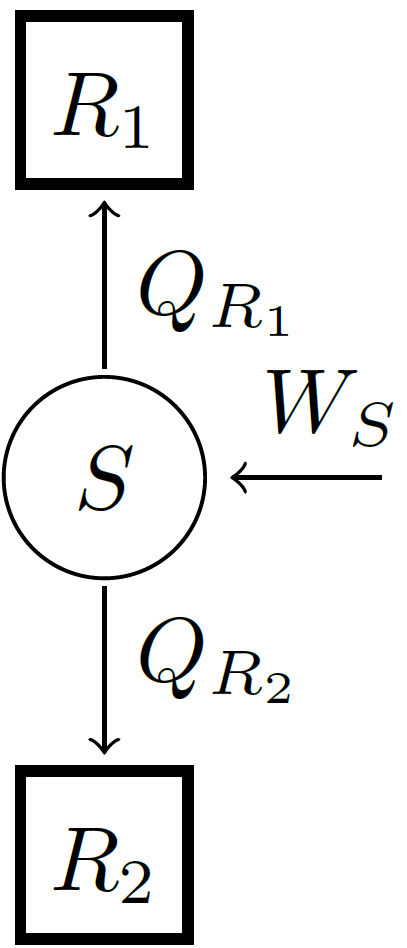
\includegraphics[width=0.9\textwidth]{Bilder/Carnot_Thm.png}
    \end{center}
\end{minipage} \hspace{2pt}
\begin{minipage}{0.39\textwidth}
    Ein System $S \in \S$, von nun an als "Maschine" bezeichnet, operiert
    zyklisch zwischen zwei Reservoirs $R_1,R_2 \in \S$, welche nicht
    Kopien voneinander sein müssen. Auf $S \vee R_1 \vee R_2$ findet also
    ein Arbeitsprozess $p \in \P_{S \vee R_1 \vee R_2}$ statt, der zyklisch
    auf $S$ ist. Ausserdem wird nur direkt in $S$ Arbeit investiert respektive
    von $S$ extrahiert, nämlich $W_S := W_S (p)$. Für die Reservoirs soll
    gelten $W_{R_1}(p) = W_{R_2}(p) = 0$. Wir betrachten die Wärmeflüsse zu
    den Reservoirs, $Q_{R_1} := Q_{R_1}(p)$ und $Q_{R_2} := Q_{R_2}(p)$, wobei
    wir annehmen, dass diese nicht null sind.
\end{minipage}

\begin{bemerkung}
    Wegen dem 1. Hauptsatz und der Zyklizität des Prozesses auf $S$ folgt
    $W_S = - Q_S$. Weiter gilt wegen $W_{R_1}(p) = W_{R_2}(p) = 0$:
    \begin{align*}
        W_S = W_{S \vee R_1 \vee R_2} = \Delta U_{S \vee R_1 \vee R_2}
    = \Delta U_{R_1} + \Delta U_{R_2} = Q_{R_1} + Q_{R_2}
    \end{align*}
\end{bemerkung}

\begin{lemma}
    Wir betrachten eine Situation wie oben beschrieben. Insbesondere sind
    nicht beide Wärmeflüsse $Q_{R_1}$ und $Q_{R_2}$ gleichzeitig null. Für
    alle solchen $p \in \P_{S \vee R_1 \vee R_2}$ gelten folgende Aussagen:
    \begin{enumerate}[(i)]
        \item $Q_{R_1} \leq 0$ und $Q_{R_2} \leq 0$ können nicht gleichzeitig gelten.
        \item Falls $p$ zusätzlich reversibel ist, so gilt $\frac{Q_{R_1}}{Q_{R_2}} < 0$.
    \end{enumerate}
\end{lemma}

\paragraph{Carnots Theorem}
Betrachte eine zyklische Maschine $S \in \S$, die unter dem reversiblen
Prozess $p \in \P_{S \vee R_1 \vee R_2}$ zwischen zwei Reservoirs $R_1,R_2
\in \S$ operiert. Die Einschränkungen seien wie oben beschrieben. Sei $S' \in
\S$ eine weitere solche Maschine, die unter $p' \in \P_{S' \vee R_1 \vee R_2}$
zwischen identischen Reservoirs operiert, jedoch nicht unbedingt reversibel.
Es ist immer mindestens ein Wärmefluss positiv nach obigem Lemma. Wir wählen
o.B.d.A. $Q_{R_2}(p') > 0$. Wir wählen die Richtung des reversiblen Prozesses
so, dass er in die gleiche Richtung arbeitet, das heisst $Q_{R_2} > 0$. Dann
gilt:
\begin{enumerate}[(i)]
    \item Die Verhältnisse der Wärmeflüsse erfüllen:
        \begin{align*}
            - \frac{Q_{R_1}(p')}{Q_{R_2}(p')} \leq - \frac{Q_{R_1}(p)}{Q_{R_2}(p)}
            := \tau(R_1,R_2) > 0
        \end{align*}
        mit Gleichheit falls $p'$ reversibel ist.
    \item Das Verhältnis $- \frac{Q_{R_1}(p)}{Q_{R_2}(p)}$ für die reversible
        Maschine hängt nur von den beiden Reservoirs $R_1$ und $R_2$ ab und
        nicht von der verwendeten zyklischen Maschine $S$ oder vom genauen
        Prozess $p$. Es ist in diesem Sinne universell.
\end{enumerate}
Eine äquivalente Beschreibung ist:
\begin{enumerate}[]
    \item $\exists \tau(R_1,R_2) \rightarrow \R$ s.d. $\forall S$ und
        $\forall p \in \P_{S \vee R_1 \vee R_2}$ zyklisch auf $S$ mit
        $Q_{R_2}(p) > 0$ gilt $- \frac{Q_{R_1}(p)}{Q_{R_2}(p)} \leq
        \tau(R_1,R_2) > 0$ mit gleichheit falls $p$ reversibel ist.
\end{enumerate}

\subsection{Absolute Temperatur}

\begin{definition}[$\tau$]
    Für das Verhältnis der mit einer nicht-trivialen reversiblen zyklischen
    Maschine ausgetauschten Wärmeflüsse mit zwei Reservoirs $R_1$ und $R_2$,
    definieren wir die Funktion
    \begin{align*}
        \tau(R_1,R_2) := - \frac{Q_{R_1}}{Q_{R_2}}
    \end{align*}
    Dabei sei $Q_{R_2} > 0$ der positive Wärmefluss. Es gilt $\tau > 0$.
\end{definition}

\begin{lemma}
    Seien $R_1,R_2,R_2$ drei beliebige verschiedene Reservoirs. Dann gilt:
    \begin{enumerate}[(i)]
        \item $\tau(R_1,R_2) \tau(R_2,R_3) = \tau(R_1,R_3)$
        \item $\tau(R,R) = 1$
        \item $\tau(R_1,R_2) = \klammer{\tau(R_2,R_1)}^{-1}$
    \end{enumerate}
\end{lemma}

\begin{definition}[Absolute Temperatur]
    Wir wählen ein beliebiges aber fixes "Referenz-Reservior" $R_{ref} \in
    \mathcal{R}$ sowie eine beliebige fixe positive Konstante $T_{ref} \in
    \R_{>0}$. Die absolute Temperatur eines Reservoirs $R$ ist definiert als
    \begin{align*}
        T := \tau(R,R_{ref}) T_{ref}
    \end{align*}
\end{definition}

\begin{lemma}
    Allgemein: $T_2 = \tau(R_2,R_1)T_1$ und somit
    $\tau(R_2,R_1) = \frac{T_2}{T_1}$.
\end{lemma}

\begin{definition}[Wärmekraftmaschine und Wärmepumpe]
    Wir nennen eine zyklische Maschine $S$, die zwischen zwei Reservoirs
    arbeitet eine Wärmekraftmaschine, falls sie Arbeit produziert, falls also
    Arbeit extrahiert werden kann. In unserer Konvention heisst das $W_S < 0$. Falls das
    umgekehrte der Fall ist, $W_S > 0$, wird Arbeit benutzt, um die Wärme vom
    kälteren ins heissere Wärmebad zu transportieren. In diesem Fall nennen
    wir die Maschine eine Wärmepumpe.
\end{definition}

\begin{definition}[Wirkungsgrad $\eta$]
    Die Effizienz einer nicht-trivialen reversiblen zyklischen Wärmekraftmaschine
    $S$, definiert als $\eta := \frac{\abs{W_S}}{\abs{Q_{R_1}}}$, wobei $Q_{R_1}$
    der negativen Wärmefluss ist, kann geschrieben werden als $1 - \frac{T_2}{T_1}$,
    wobei $T_1 > T_2$ die Temperaturen der beiden Reservoirs sind, die die
    Maschine nutzt um Arbeit zu produzieren. Eine beliebige andere
    Wärmekraftmaschine (nicht unbedingt reversible) kann höchstens diese
    Effizienz erreichen. Die maximale Effizienz $\eta_C := 1 - \frac{T_2}{T_1}$,
    auch Carnot Effizienz genannt, hängt also nur von den Temperaturen der
    involvierten Reservoirs ab.
\end{definition}

\begin{definition}[Leistungszahl]
    Für die Wärmepumpen kann man eine analoge Aussage machen. Die Leistungszahl
    (auch Heizzahl oder Coefficient of Performance COP) einer Wärmepumpe ist
    definiert als das Verhältnis der von der Maschine abgegebene Wärme zu
    investierter Arbeit. Die Leistungszahl ist von oben beschränkt:
    \begin{align*}
        \text{COP} := \frac{Q_{R_2}}{W_S} \leq \frac{1}{1 - \frac{T_1}{T_2}}
    \end{align*}
\end{definition}

\paragraph{0. Hauptsatz}
Zwei Reservoirs $R_1$ und $R_2$ sind im Gleichgewicht, wenn $\tau(R_1,R_2)
= 1$, also wenn sie die gleiche Temperatur haben. Wir schreiben $R_1 \sim R_2$.
Insbesondere identische Reservoirs $R \cong R'$ erfüllen $R \sim R'$. Der
0. Hauptsatz besagt: Wenn System $A$ und $B$ im thermischen Gleichgewicht
sind und Systeme $B$ und $C$ ebenfalls, dann sind auch $A$ und $C$ im
thermischen Gleichgewicht.

\begin{definition}[Temperatur eines Wärmeflusses]
    Sei $S = S_1 \vee S_2 \in \S$ ein disjunkt bipartites System, auf welchem
    ein Arbeitsprozess $p \in \P_S$ ausgeführt wird. Wir schreiben $W_i :=
    W_{S_i}(p)$ und $Q := Q_{S_2}(p)$. Für $Q \neq 0$ sagen wir, die Wärme
    zwischen $S_1$ und $S_2$ fliesst bei Temperatur $T$, falls zwei Reservoirs
    $R_1$ und $R_2$, beide bei Temperatur $T$, zusammen mit zwei Prozessen
    $p_1 \in \P_{S_1 \vee R_1}$ und $p_2 \in \P_{S_2 \vee R_2}$ existieren,
    so dass $W_{S'}(p_i) = W_{S'}(p)$ für alle Systeme $S' \in \S$ welche
    keinen Überlapp mit dem anderen System haben, $S' \wedge S_{i+1} = \emptyset$,
    und die Zustandsänderungen auf den $S_i$ unter $p_i$ beibehalten werden,
    $\floor{p_i}_{S_i} = \floor{p}_{S_i}$ sowie $\ceil{p_i}_{S_i} = \ceil{p}_{S_i}$.
\end{definition}

\begin{lemma}
    Wenn man dem Wärmefluss eine Temperatur zuordnen kann, sind die
    Teilprozesse $p_i \in \P_{S_i \vee R_i}$ reversibel und die Temperatur
    des Wärmeflusses eindeutig.
\end{lemma}


\subsection{Clausius' Theorem und Entropie}

Aus vorherigen Erkentnissen folgt: $- \frac{Q_1}{Q_2} = \frac{T_1}{T_2}
\Leftrightarrow \frac{Q_1}{T_1} + \frac{Q_2}{T_2} = 0$ für reversible
Prozesse. Allgemein folgt:

\paragraph{Clausius' Theorem}
Sei $S \in \S$ ein beliebiges System und $\geschwungeneklammer{R_i}_{i=1}^N$
eine Menge von Reservoirs, so dass $R_i$ die Temperatur $T_i$ hat. Für jedes
$i=1,\dots,N$ sei $p_i \in \P_{S \vee R_i}$ ein Arbeitsprozess auf $S$ und
dem Reservoir $R_i$ mit $W_{R_i}(p_i) = 0$, so dass der Prozess $p := p_N
\circ \dotsb \circ p_1$ definiert ist und insgesamt zyklisch auf $S$. Dann gilt
\begin{align*}
    \sum_i \frac{Q_S (p_i)}{T_i} \leq 0
\end{align*}
mit Gleichheit wenn $p$ reversibel ist.
Für quasistatische Prozesse wie im Clausius Theorem beschrieben gilt:
\begin{align*}
    \oint \frac{\delta Q_s}{T} \leq 0
\end{align*}
wieder mit Gleichheit falls $p$ reversibel ist.

\begin{definition}[Entropie]
    Sei $S \in \S$ ein System und $\sigma_{ref} \in \Sigma_S$ ein beliebiger
    aber fixer Zustand darauf. Sei $S_{ref} \in \R$ eine beliebige reelle
    Konstante. Für einen Zustand $\sigma \in \Sigma_S$ definieren wir die
    Entropie
    \begin{align*}
        S_S (\sigma) := \sum_{i=1}^N \frac{Q_S (p_i)}{T_i} + S_{ref}
    \end{align*}
    wobei die Summe über die reversiblen Teilprozesse $p_i$ wie im Clausius
    Theorem geht, so dass das System $S$ während den $p_i$ die Wärme $Q_S(p_i)$
    bei Temperatur $T_i$ austauscht und $p = p_N \circ \dotsb \circ p_1$ so ist,
    dass $\floor{p}_S = \sigma_{ref}$ und $\ceil{p}_S = \sigma$. Falls die
    beteiligten Prozesse quasistatisch sind, kann man die Definition auch
    schreiben als
    \begin{align*}
        S_S (\sigma) := \int_{\sigma_{ref}}^\sigma \frac{\delta Q_S}{T} + S_{ref}
    \end{align*}
    Wir definieren das exakte Differential $dS = \frac{\delta Q_S}{T}$.
\end{definition}

\begin{theorem}[Entropiesatz]
    In einem adiabatischen Prozess kann die Entropie eines Systemes nicht
    abnehmen, d.h. für einen adiabatischen Prozess $p \in \P$ auf einem
    System $S$ gilt:
    \begin{align*}
        \Delta S_S (p) \geq 0
        \hspace{20pt} \Leftrightarrow \hspace{20pt}
        S_S(\floor{p}_S) \leq S_S(\ceil{p}_S)
    \end{align*}
    und es gilt Gleichheit, falls der Prozess reversibel ist.
\end{theorem}

\begin{bemerkung}
    Mit unserem bisherigen Wissen folgern wir, dass
    \begin{align*}
        dU = T dS - p dV
    \end{align*}
    Während einem Prozess, in dem dass das Volumen $V$ konstant gehalten wird,
    gilt dann
    \begin{align*}
        T = \frac{\partial U}{\partial S} \Big|_V
    \end{align*}
    Da $T$ ausgedrückt werden kann durch Zustandsgrössen, ist $T$ also eine
    Zustandsgrösse und wird Temperatur des Systems genannt.
\end{bemerkung}


\section{Die thermodynamischen Potentiale}

\subsection{Skalierung von Systemen}

Die positive Zahl $\lambda \in \R_{>0}$ sei der Skalierungsfaktor. Sei hier
$\lambda = 2$. Weiter sei $S \in \S$ ein System, welches wir skalieren, also
um den Faktor $\lambda = 2$ vergrössern möchten. Die Beschreibung des
skalierten Systemes, welches fortan $2S$ genannt wird, ist dann eine
"eingeschränkte Beschreibung" von $S \vee S'$, wobei $S' \cong S$ eine
Kopie von $S$ ist. Für $2S$ sollen nicht alle Zustände und Prozesse erlaubt
sein, die auf $S \vee S'$ möglich sind.
\begin{enumerate}[(i)]
    \item Die Zustände von $2S$ sind von der Form $\sigma \vee \sigma'$,
        wobei $\sigma \in \Sigma_S$ und $\sigma' \in \Sigma_{S'}$ der zu
        $\sigma$ äquivalente Zustand ist. D.h. der Zustandsraum ist
        $\Sigma_{2S} = \geschwungeneklammer{\sigma \vee \sigma' \ | \
        \sigma \in \Sigma_S , \ \sigma \cong \sigma' \in \Sigma_{S'}}$.
    \item Genauso sind die Prozesse auf $2S$ von der Form $p \vee p'$, wobei
        $p' \cong p$ der zu $p$ äquivalente Prozess ist. Insbesondere ist
        die Menge der Arbeitsprozesse auf $2S$ gleich $\P_{2S} =
        \geschwungeneklammer{p \vee p' \ | \ p \in \P_S , \ p \cong p' \in
        \P_{S'}}$.
\end{enumerate}
Ein allgemeiner Prozess auf $2S$ wird also den Zustandsraum $\Sigma_{2S}$
respektieren, d.h. er darf Zustände der Form $\sigma_1 \vee \sigma_1'$ nur
solche der Form $\sigma_2 \vee \sigma_2'$ überführen. Im Zusammenhang mit
skalierten Systemen schreiben wir ab jetzt $2\sigma := \sigma \vee \sigma'$
für Zustände auf $2S$. Gleiches foll für Arbeitsprozesse gelten,
$2p := p \vee p'$.

Äquivalent: Ein um den Faktor $\lambda \in \N$ skaliertes System vom System
$S$ ist $S^{(1)} \vee \dotsb \vee S^{(\lambda)}$ mit $S \cong S^{(i)} \ \forall
i =1,\dots,\lambda$. Falls $\lambda = \frac{1}{\nu}$ für ein $\nu \in \N$,
wird $\lambda \sigma$ definiert als der folgende Zustand:
\begin{align*}
    \underbrace{\lambda \sigma \vee \dotsb \vee \lambda \sigma}_{\nu \text{ mal}}
    = \sigma
\end{align*}
Für $\lambda = \frac{\mu}{\nu}$ definiert man $\lambda \sigma = \mu
\klammer{\frac{1}{\nu} \sigma}$. Da $\Q$ dicht ist in $\R$ folgt die
Aussage für beliebige $\lambda \in \R$.

\begin{definition}[Homogene Zustandsvariablen]
    Sei $S \in \S$ und $X_S$ eine Zustandsvariable von $S$, welche
    für beliebige $\lambda \in \R$ zugehörige Zustandsgrössen $X_{\lambda S}$
    auf den skalierten Systemen $\lambda S$ kennt. Eine solche Zustandsvariable
    heisst homogen vom Grad $k$ falls
    \begin{align*}
        X_{\lambda S} (\lambda \sigma) = \lambda^k X_{S} (\sigma)
    \end{align*}
    für alle $\sigma \in \Sigma_S$ und alle $\lambda \in \R$. Zustandsgrössen,
    die homogen vom Grad $0$ sind, heissen intensiv. Solche, die homogen
    vom Grad $1$ sind, heissen extensiv.
\end{definition}


\subsection{Das Extremalprinzip für die Entropie}

Betrachte ein zusammengesätztes System $S = S' \vee S''$, welches zunächst
in einem Zustand $\sigma' \vee \sigma''$ ist. Zunächst sind $S'$ und $S''$
nicht im thermischen Kontakt. Für die Entropie des Anfangszustands
$\sigma' \vee \sigma''$ gilt:
\begin{align*}
    S_S(\sigma' \vee \sigma'') = S_{S'} (\sigma) + S_{S''} (\sigma'')
\end{align*}
$\sigma' \vee \sigma''$ wird manchmal gehemmter Gleichgewichtszustand genannt.
Entfernen der Trennwand ist ein Arbeitsprozess auf $S$, wenn $S$ ansonsten
isoliert ist, der keine Arbeit kostet. Wir bezeichnen den Endzustand nach
Entfernen der Trennwand mit $\sigma' + \sigma''$. Der Endzustand wird als
vollständiges Gleichgewicht bezeichnet. Nach dem Entropiesatz gilt für
Arbeitsprozesse (insbesondere adiabatische Prozesse): $S_S (\sigma' \vee
\sigma'') \leq S_S (\sigma' + \sigma'')$ und Gleichheit falls das Entfernen
der Wand reversibel ist.

\begin{theorem}[Extremalprinzip der Entropie]
    Für $S \in \S$ und $\sigma \in \Sigma_S$ sowie jede mögliche disjunkte
    Aufteilung von $S$ in Subsysteme $S',S'' \in \S$ ($S = S' \vee S''$)
    gilt
    \begin{align*}
        S_S (\sigma) \max_{\stackrel{\sigma',\sigma''}{\sigma' + \sigma'' = \sigma}}
            S_{S'} (\sigma') + S_{S''}(\sigma'')
    \end{align*}
    wobei die Zustände $\sigma' \in \Sigma_{S'}$ und $\sigma'' \in \Sigma_{S''}$
    Zustände der Systeme $S'$ und $S''$ sein sollen. Informell heisst das,
    dass in einem abgeschlossenen System die Entropie maximal ist, wenn
    der Gesamtzustand im Gleichgewicht ist.
\end{theorem}

\subsection{Homogenität}

Für einen Arbeitsprozess, bei dem sowohl Substanzmenge als auch Volumen
verändert werden können, soll von nun an gelten, dass
\begin{align*}
    \delta W = - p dV + \mu d N
\end{align*}
Die neue Grösse $\mu$, die eine Zustandsgrösse ist, heisst chemisches Potential.
Wir können weiter herleiten:

\begin{align*}
    dS = \frac{1}{T} \klammer{dU + p dV - \mu dN}
\end{align*}
Daraus folgt:
\begin{align*}
    \frac{\partial S}{\partial U} \Big|_{V,N} = \frac{1}{T}
    \hspace{15pt} , \hspace{15pt}
    \frac{\partial S}{\partial V} \Big|_{U,N} = \frac{p}{T}
    \hspace{15pt} , \hspace{15pt}
    \frac{\partial S}{\partial N} \Big|_{U,V} = - \frac{\mu}{T}
\end{align*}

\paragraph{Homogenitätsrelation}
\begin{align*}
    S = U \frac{\partial S}{\partial U} \Big|_{V,N} +
        V \frac{\partial S}{\partial V} \Big|_{U,N} +
        N \frac{\partial S}{\partial N} \Big|_{U,V}
    = \frac{1}{T} \klammer{U + p V - \mu N}
\end{align*}


\subsection{Konkavität der Entropie}

Betrachte $\alpha',\alpha'' \in \R$ mit $\alpha' + \alpha'' = 1$. Seien
$\sigma' \in \Sigma_{S'}$ und $\sigma'' \in \Sigma_{S''}$ Zustände auf $S'$
respektive $S''$ und damit $\alpha' \sigma' \in \Sigma_{\alpha' S'}$ und
$\alpha'' \sigma'' \in \Sigma_{\alpha'' S''}$ wieder Zustände auf $\alpha' S'$
respektive $\alpha'' S''$. Dann gilt gemäss dem Extremalprinzip und der
Extensivität der Entropie, dass
\begin{align*}
    S(\alpha' \sigma' + \alpha'' \sigma'') \geq
    \alpha' S(\sigma') + \alpha'' S(\sigma'')
\end{align*}

\begin{theorem}[Äquivalenz von Eigenschaften der Entropie]
    Folgende Aussagen sind äquivalent:
    \begin{enumerate}[(i)]
        \item $S(\sigma)$ ist linear zwischen $\sigma'$ und $\sigma''$.
        \item $S(\sigma' + \sigma'') = S(\sigma') + S(\sigma'')$, d.h.
            $\sigma'$ und $\sigma''$ sind im vollständigen Gleichgewicht.
        \item $\mathbf{\nabla} S(\sigma') = \mathbf{\nabla} S(\sigma'')$, d.h
            für $\sigma = (U,V,N)$ gilt $T' = T''$, $p' = p''$ und $\mu' = \mu''$.
            Hier ist:
            \begin{align*}
                \mathbf{\nabla} S(\sigma) = \begin{pmatrix}
                    \frac{\partial S}{\partial U} \Big|_{V,N} &
                    \frac{\partial S}{\partial V} \Big|_{U,N} &
                    \frac{\partial S}{\partial N} \Big|_{U,V}
                \end{pmatrix}
            \end{align*}
    \end{enumerate}
\end{theorem}

\begin{theorem}[Gibbs-Duhem Relation]
    Es gilt:
    \begin{align*}
        S dT - V dp + N d \mu = 0
    \end{align*}
    Insbesondere sind nur zwei der drei Zustandsgrössen $T,p$ und $\mu$
    unabhängig.
\end{theorem}

\subsection{Stabilitätsbedingungen}

Konkavität der Entropie ist gleichbedeutend damit, dass die Hesse-Matrix
\begin{align*}
    \partial^2 S = \begin{pmatrix}
        \frac{\partial^2 S}{\partial U^2} &
        \frac{\partial^2 S}{\partial U \partial V} \\
        \frac{\partial^2 S}{\partial V \partial U} &
        \frac{\partial^2 S}{\partial V^2}
    \end{pmatrix}
\end{align*}
in jedem Punkt $(U,V,N=1)$ negativ semidefinit ist. Insbesondere:
\begin{align*}
    \frac{\partial^2 S}{\partial U^2} \leq 0
    \hspace{10pt} , \hspace{10pt}
    \det (\partial^2 S) \geq 0
\end{align*}

\begin{definition}[Wärmekapazität und Kompressibilität]
    Die spezifische Wärme für festes Volumen $V$ und diejenige für
    festen Druck $p$ sind:
    \begin{align*}
        C_V :=& \frac{\delta Q}{\partial T} \Big|_{V}
        = \frac{\partial U}{\partial T} \Big|_{V}
        \\
        C_p :=& \frac{\delta Q}{\partial T} \Big|_{p}
            = T \frac{\partial S}{\partial T} \Big|_{p}
            = \frac{\partial U + p \partial V}{\partial T} \Big|_{p}
            = \frac{\partial U}{\partial T} \Big|_{p} + p \frac{\partial V}{\partial T} \Big|_{p}
    \end{align*}
    Die isotherme Kompressibilität ist definiert als
    \begin{align*}
        \kappa_T := - \frac{1}{V} \frac{\partial V}{\partial p} \Big|_{T}
    \end{align*}
    Es gilt $C_V \geq 0, \kappa_T \geq 0$ und $C_p \geq 0$. Weiter gilt:
    \begin{align*}
        C_p - C_V = \frac{T V \alpha^2}{\kappa_T} \geq 0
    \end{align*}
    mit $\alpha = \frac{1}{V} \frac{\partial V}{\partial T} \Big|_p$.
\end{definition}


\subsection{Weitere thermodynamischen Potentiale}

\subsubsection{Die Legendre Transformation}

\begin{definition}[Legendretransformierte]
    Sei $D \subset \R^n$ und $f: D \rightarrow \R$. Die Legendretransformierte
    $f^\ast$ von $f$ ist definiert für jene $p \in \R^n$, für welche
    \begin{align*}
        f^\ast (p) = \sup_{x \in D} \klammer{ p \cdot x - f(x)}
    \end{align*}
    endlich ist. Wir nennen den Definitionsbereich $D^\ast$.
\end{definition}

\begin{theorem}
    Sei $f: D \rightarrow \R$ eine reelle Funktion. Dann gilt:
    \begin{enumerate}[(i)]
        \item $f^\ast : D^\ast \rightarrow \R$ ist konvex.
        \item Ist $f$ konvex, so ist $f^{\ast \ast} = f$ (mit $D^{\ast \ast} = D)$
        \item Ist $f=f(x,y)$ konvex in $(x,y)$, so ist $f^\ast (p,y)$ konkav in $y$.
            \begin{align*}
                f^\ast (p,y) = \sup_x \eckigeklammer{p \cdot x - f(x,y)}
            \end{align*}
    \end{enumerate}
    Ist $f(S,V,N)$ konvex, so ist $f^{\ast(S \rightarrow T)} (T,V,N)$ konvex in
    $T$ und konkav in allen anderen Variablen.
\end{theorem}

\begin{bemerkung}
    Ist $f$ differenzierbar und konvex, so gelten
    \begin{align*}
        \klammer{f^\ast}'(p_0) = x_0
        \hspace{10pt} , \hspace{10pt}
        \klammer{f^\ast}' = \klammer{f'}^{-1}
    \end{align*}
    Falls $f$ strikt konvex und differenzierbar ist, gilt sogar
    \begin{align*}
        x_0 = \klammer{f'}^{-1} (p_0)
    \end{align*}
\end{bemerkung}

\subsubsection{Energie}

Homogenitätsrelation: $U = T S - p V + \mu N$. $U(S,V,N)$ ist konvex in $S,V$
und $N$. Insbesondere gilt:
\begin{align*}
    dU = T dS - p dV + \mu dN
\end{align*}
Daraus folgt:
\begin{align*}
    \frac{\partial U}{\partial S} \Big|_{V,N} = T
    \hspace{10pt} , \hspace{10pt}
    \frac{\partial U}{\partial V} \Big|_{S,N} = -p
    \hspace{10pt} , \hspace{10pt}
    \frac{\partial U}{\partial N} \Big|_{S,V} = \mu
\end{align*}

\subsubsection{Die (Helmholtz) freie Energie}
\begin{align*}
    F(T,V,N) = U(S,V,N) - T S = - p V + \mu N
\end{align*}
wobei $S$ als Lösung von $\frac{\partial U}{\partial S} \Big|_{V,N} = T$
aufgefasst wird. $F$ ist homogen vom Grad $1$ in $V$ und $N$. Weiter folgt:
\begin{align*}
    dF = dU - T dS - S dT
    = -p dV + \mu dN - S dT
\end{align*}
Daraus folgt:
\begin{align*}
    \frac{\partial F}{\partial T} \Big|_{V,N} = -S
    \hspace{10pt} , \hspace{10pt}
    \frac{\partial F}{\partial V} \Big|_{T,N} = -p
    \hspace{10pt} , \hspace{10pt}
    \frac{\partial F}{\partial N} \Big|_{T,V} = \mu
\end{align*}
$F(T,V,N)$ ist konkav in $T$ und konvex in $(V,N)$.

\paragraph{Extremalprinzip für Helmholtz freie Energie}
Bei fixem Gesamtvolumen, fixer Gesamtstoffmenge und fixer Temperatur ist $F$
im Gleichgewicht minimal.

\paragraph{Maxwell-Relationen}
Folgen aus $\frac{\partial^2 F}{\partial T \partial V} =
\frac{\partial^2 F}{\partial V \partial T}$ und anderen partiellen
Ableitungen.
\begin{align*}
    \frac{\partial S}{\partial V} \Big|_{T,N}
    = \frac{\partial p}{\partial T} \Big|_{V,N}
    \hspace{5pt} , \hspace{5pt}
    - \frac{\partial p}{\partial N} \Big|_{T,V}
    = \frac{\partial \mu}{\partial V} \Big|_{T,N}
    \hspace{5pt} , \hspace{5pt}
    - \frac{\partial S}{\partial N} \Big|_{T,V}
    = \frac{\partial \mu}{\partial T} \Big|_{V,N}
\end{align*}

\subsubsection{Die Enthalpie}
\begin{align*}
    H(S,p,N) = U(S,V,N) + p V = T S + \mu N
\end{align*}
wobei $V$ eine Lösung von $\frac{\partial U}{\partial V} \Big|_{S,N} = -p$ ist.
Weiter folgt:
\begin{align*}
    dH = dU + p dV + V dp = T dS + V dp + \mu dN
\end{align*}

\subsubsection{Die Gibbs'sche freie Energie}
\begin{align*}
    G(T,p,N) &= U(T,p,N) - T S(T,p,N) + p V(T,p,N)
    \\
    &= F(T,p,N) + p V(T,p,N) = H(T,p,N) - T S
    \\
    &= \mu(T,p) N 
    \\
    dG &= dU - d(TS) + d(pV) = -S dT + V dp + \mu dN
\end{align*}

\subsubsection{Das Grosskanonische Potential}
\begin{align*}
    \Omega(T,V,\mu) &= U(S,V,N) - T S - \mu N
    = F(T,V,N) - \mu N
    = -p(T,\mu) V
    \\
    d \Omega &= - S dT - p dV - N d \mu
\end{align*}

\subsection{Konkavität, Konvexität und Extremalprinzip}

Die freie Energie $F(T,V,N)$ ist konkav in $T>0$ und konvex in $(V,N)$.
Die Enthalpie $H(S,p,N)$ ist konkav in $p$ und konvex in $(S,N)$.
Die Gibbs'sche freie Energie $G(T,p,N)$ ist konkav in $(T,p)$ und linear in $N$.
Das Grosskanonische Potential $\Omega(T,V,\mu)$ ist konkav in $(T,\mu)$ und
linear in $V$.

\paragraph{Extremalprinzip der freien Energie}
"Bei bestem Gesamtvolumen und fester Temperatur ist die freie Energie im
vollständigen Gleichgewicht minimal."
\begin{align*}
    F(T,V',N') + F(T,V'',N'') \geq F(T,V' + V'' , N' + N'')
\end{align*}


\subsection{Reine und gemischte Phasen}

Angenommen jeder Zustand $\sigma = (U,V)$ zu einem $(T,p)$ ist eindeutig
darstellbar als "Mischung" $\sigma = \sum_{i}^N \alpha_i \sigma_i$ mit $\alpha_i
\geq 0 \ \forall i$ und $\sum_{i}^N \alpha_i = 1$ wobei $N=1,2,3$.

Die Extremalpunkte der konvexen Berührungsfigur (hier $\sigma_1,\sigma_2,
\sigma_3$) heissen reine Phasen. Diese Punkte sind definiert als diejenigen
Zustände, die nicht innerhalb der Verbindungsstrecke von zwei anderen Punkten
liegen und man somit nicht als echte Mischung von zwei Zuständen zum selben
$(T,p)$ auffassen kann.

\paragraph{Gibbs'sche Phasenregel}

Die Gibbs'sche Phasenregel besagt, dass die Berührungsflächen
Simplices\footnote{Ein Simplex ist ein $n$-dimensionales Polytop mit
$n+1$ Ecken (Extremalpunkte). Dies ist die kleinste Anzahl Ecken, die
ein $n$-dimensionales Polytop haben kann.} sind. Sei nun $n$ die Anzahl
koexistierender Phasen in einer Mischung und $f$ die Anzahl freier intensiver
Grössen bei festem $n$. Dann besagt die Gibbs'sche Phasenregel ferner, dass
Simplizes in Scharen vorkommen: Für ein System mit zwei Koordinaten $(U,V)$
ist
\begin{align*}
    f = 3 - n
\end{align*}

\begin{figure}[h]
    \centering
    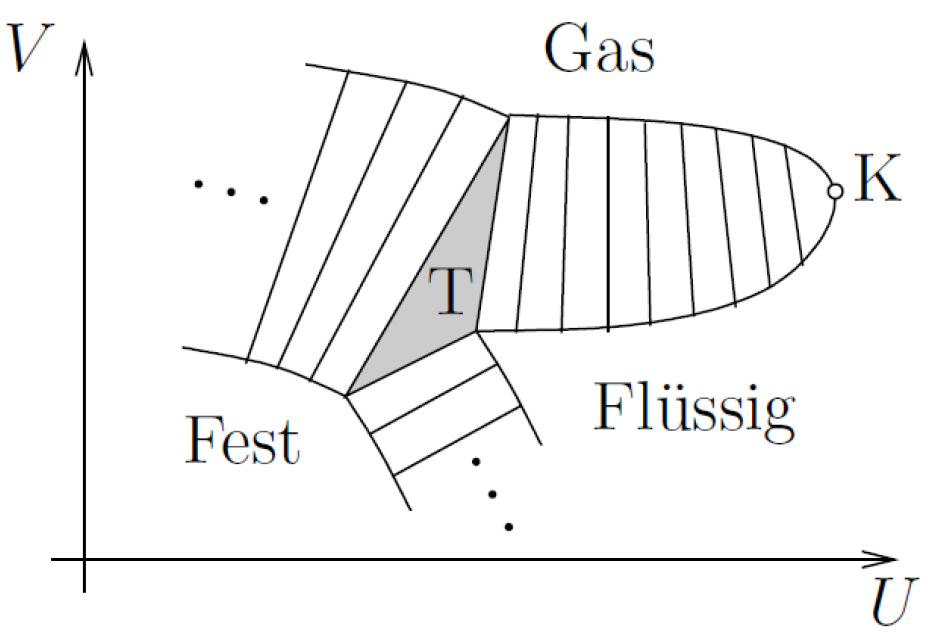
\includegraphics[width=0.25\textwidth]{Bilder/Gibbs_UV.png}
    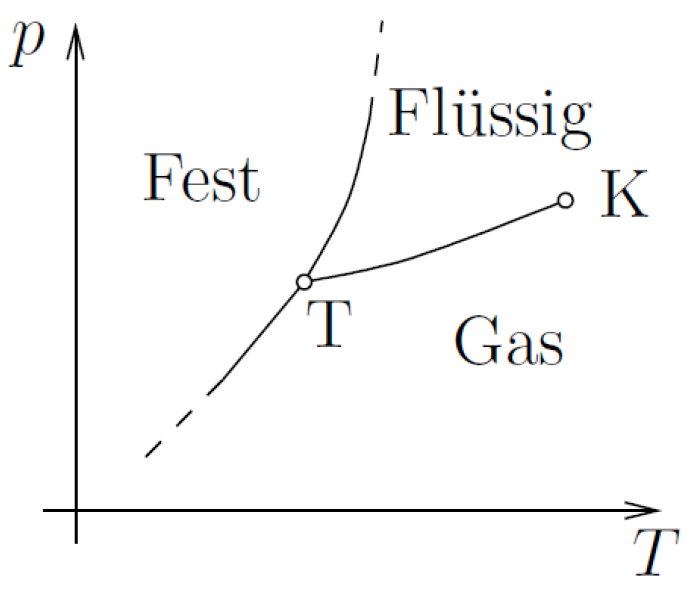
\includegraphics[width=0.2\textwidth]{Bilder/Gibbs_Tp.png}
    \caption{Links: Entropiefläche (Ansicht von oben) im $U-V$ Diagramm.
        Rechts: Das zugehörige $p-T$ Phasendiagramm.}
    \label{Gibbs}
\end{figure}

Die weissen Gebiete im $U-V$ und im $p-T$ Diagramm entsprechen reinen Phasen:
Die Entropie ist dort strikt konkav und der Zusammenhang $(U,V) \leftrightarrow
(T,p)$ bijektiv. Bei einem Phasenübergang $n$-ter Ordnung ist $G$ als Funktion
von $T$ und $p$ in seinen ersten $n-1$ Ableitungen stetig, die $n$-te
Ableitung ist stetig. Ein erster Ordnung Phasenübergang involviert generell
latente Wärme, d.h. es wird Energie vom System aufgenommen oder abgegeben,
ohne dass dies eine Temperaturänderung zur Folge hat.

\paragraph{Gleichung von Claisius-Clapeyron}
\begin{align*}
    \frac{\partial p}{\partial T} \equiv
    \frac{\partial p}{\partial T} \Big|_{V,N}
    = \frac{\partial S}{\partial V} \Big|_{T,N}
    = \frac{S_2 - S_1}{V_2 - V_1}
    = \frac{L_{12}}{T (V_2 - V_1)}
\end{align*}
Da $\frac{\partial p}{\partial T}$ unabhängig ist von $V$, muss auch
$\frac{\partial S}{\partial V} \Big|_{T,N}$ unabhängig von $V$ sein. Also ist
$S$ linear in $V$. $L_{12}$ ist die Übergangswärme von Phase 1 zu Phase 2.
Es gilt:
\begin{align*}
    L_{12} := \int_{\sigma_1}^{\sigma_2} \delta Q
    = \int_{\sigma_1}^{\sigma_2} T dS = T (S_2 - S_1)
\end{align*}
Für ein Wasser-Eis Gemisch ist $L_{12} > 0$, aber $V_2 - V_1 < 0$ und
somit $\frac{\partial p}{\partial T} < 0$. Also kann bei isothermer
Druckzunahme Eis schmelzen.



\section{Mehrstoffsysteme}

System besteht aus $r$ Komponenten (= Stoffen). Wir betrachten nur Systeme,
welche Mischprozesse zulassen. Gemischte Zustände sind Endzustände von
Mischprozessen. Der ungemischte Zustand kann beschrieben werden durch
$\sigma_i = (U_i,V_i,N_i)$ für $i=1,\dots,r$ und der gemischte Zustand ist
gegeben durch $\sigma = (U,V,N_1,\dots,N_r)$.

\subsection{Thermodynamik von Mischungen}

\begin{minipage}{0.25\textwidth}
    \centering
    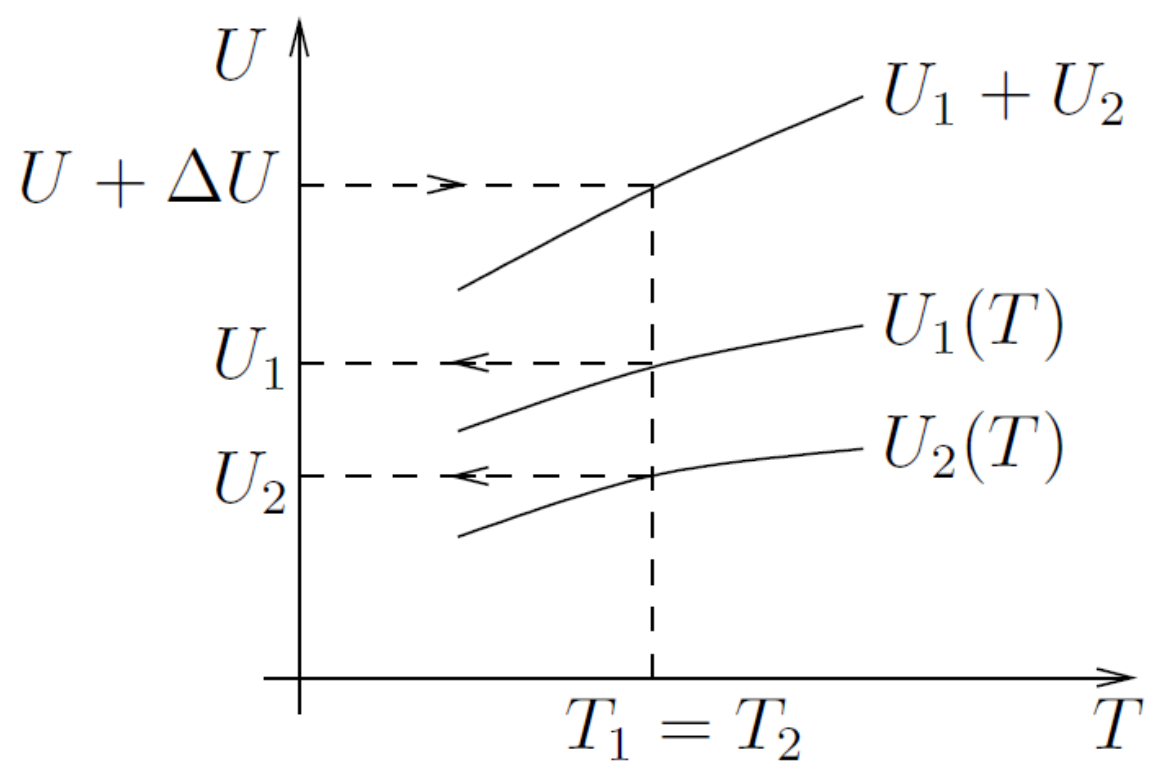
\includegraphics[width=\textwidth]{Bilder/Mehrstoffsystem_U.png}
\end{minipage}
\begin{minipage}{0.23\textwidth}
    Mischungen und Entmischungen werden durch semipermeable Wände realisiert.
    Diese Prozesse sind reversibel und kosten Arbeit. Sei $S = S_1 \vee S_2$ und
    $\Delta U$ die zugeführte Arbeit. Dann gilt:
\end{minipage}

\begin{align*}
    S_S (U,V,N_1,N_2) &= S_{S_1} (U_1,V,N_1) + S_{S_2} (U_2,V,N_2)
    \\
    U_1 + U_2 &= U + \Delta U
    \\
    T_1 &= T_2
\end{align*}
Nun können wir bereits bekanntes verallgemeinern:
\begin{align*}
    dS = \frac{1}{T} d U + \frac{p}{T} dV - \sum_{i=1}^r \frac{\mu_i}{T} d N_i
\end{align*}
Mit $p$ dem Gesamtdruck des Gemisches und $\mu_i$ den entsprechenden
chemischen Potentialen.
\begin{align*}
    \mu_i = - T \frac{\partial S}{\partial N_i} \Big|_{U,V,N_{j \neq i}}
\end{align*}
Von den $r+2$ intensiven Grössen $(T,p,\mu_1,\dots,\mu_r)$ sind nur $r+1$
frei wählbar. Insbesondere sind die $\mu_i$ intensiv und die $N_i$ extensiv.
Die chemischen Potentiale hängen nur von den Verhältnissen der $N_i$ ab:
\begin{align*}
    \mu_i = \mu_i(T,p,c_1,\dots,c_r)
    \hspace{10pt} , \hspace{10pt}
    c_i := \frac{N_i}{N}
    \hspace{10pt} , \hspace{10pt}
    N = N_1 + \dotsb + N_r
\end{align*}
Wegen $c_1 + \dotsb + c_r = 1$ sind nur $r-1$ Konzentrationen frei wählbar.
Die Gibbs'sche Phasenregel besagt neu
\begin{align*}
    f = r+2-n
\end{align*}

\paragraph{Extremalprinzip der Gibbs'schen Energie}
Da $G(T,p,N_1,\dots,N_r)$ konkav ist in $(T,p)$ und konvex in $(N_1,\dots,N_r)$
gilt:
\begin{align*}
    G'(T,p,N_1',\dots,N_r') + G'' (T,p,N_1'',\dots,N_r'') 
    \\ \geq
    G(T,p,N_1' + N_1'' ,\dots, N_r' + N_r'')
\end{align*}
Es folgt, dass im Gleichgewicht gilt: $\mu_i' = \mu_i''$.

\subsection{Ideale Mischungen}

Ideale Mischungen sind charakterisiert durch $\Delta U = 0$ und somit
\begin{align*}
    U = \sum_{i=1}^r U_i
\end{align*}
wobei $U_i = U_i (U,V,N_1,\dots,N_r)$. Weiter gilt $T_i = T_j \ \forall
i,j =1,\dots,r$ und
\begin{align*}
    S(U,V,N_1,\dots,N_r) = \sum_{i=1}^r S_i (U_i,V,N_i)
\end{align*}
Für ideale Mischungen ist die adiabatische Entmischung isotherm.
\begin{align*}
    \frac{1}{T} = \frac{\partial S}{\partial U} \Big|_{V,\geschwungeneklammer{N_k}}
    = \sum_{i=1}^r \frac{\partial S_i}{\partial U_i} \Big|_{V,N_i}
        \frac{\partial U_i}{\partial U} \Big|_{V,\geschwungeneklammer{N_k}}
    = \frac{1}{T_1} \sum_{i=1}^r \frac{\partial U_i}{\partial U} \Big|_{V,\geschwungeneklammer{N_k}}
    = \frac{1}{T_1}
\end{align*}
mit $T_1 \equiv T_i \ \forall i$ und $T$ der Temperatur des Mischung.
Für die Freie Energie gilt:
\begin{align*}
    F(T,V,N_1,\dots,N_r) = U - T S
    = \sum_{i=1}^r U_i - T \sum_{i=1}^r S_i
    = \sum_{i=1}^r F_i (T,V,N_i)
\end{align*}
Somit:
\begin{align*}
    p = - \frac{\partial F}{\partial V} \Big|_{T,N_i}
    = - \sum_{i=1}^r \frac{\partial F_i}{\partial V} \Big|_{T,N_i}
    = \sum_{i=1}^r p_i
\end{align*}
Mit $p_i$ den Partialdrücken. Dass die Summe der Partialdrücke den Gesamtdruck
der Mischung ergibt ist bekannt unter dem Namen Daltons Gesetz. Weiter gilt:
\begin{align*}
    G(T,p,N_1,\dots,N_r)
    = \sum_{i=1}^r U_i - T \sum_{i=1}^r S_i + V \sum_{i=1}^r p_i
    = \sum_{i=1}^r G_i (T,p_i,N_i)
\end{align*}
Daraus folgt:
\begin{align*}
    \frac{\partial G_i}{\partial p_i} \Big|_{T,N_i}
    &= \frac{\partial G}{\partial p} \Big|_{T,N_i}
    = V
    \\
    \frac{\partial G}{\partial N_i} \Big|_{T,p,N_{j \neq i}}
    &= \mu_i (T,p,N_1,\dots,N_r)
\end{align*}
Hier ist $\mu_i$ das chemische Potential der $i$-ten Komponente in der
Mischung. Für gegebenes $p$ und $T$ gilt $G_i (T,p_i,N_i) = G_i (T,p_i(N_1,\dots,N_r),N_i)$
und somit:
\begin{align*}
    \mu_i (T,p,N_1,\dots,N_r)
    = \mu_i^0 (T,p_i)
\end{align*}
wobei $\mu_i^0$ das chemische Potential des reinen Stoffes ist.
Im Falle eines idealen Gases gilt:
\begin{align*}
    \frac{\partial G}{\partial p} \Big|_{T,N} = V = \frac{N R T}{p}
\end{align*}
und somit:
\begin{align*}
    G_i(T,p_i,N_i) &= G_i (T,p,N_i) + \int_{p}^{p_i} \frac{\partial G_i}{\partial p'} \Big|_{T,N_i} dp'
    \\
    &= G_i (T,p,N_i) + N_i R T \log \klammer{\frac{N_i}{N}}
    \\
    \Rightarrow
    G(T,p,N_1,\dots,N_r) &= \sum_{i=1}^r G_i (T,p,N_i) + N_i R T \log \klammer{\frac{N_i}{N}}
\end{align*}
Weiter gilt:
\begin{align*}
    \mu_i(T,p,N_1,\dots,N_r) = \frac{\partial G}{\partial N_i} \Big|_{T,p}
    &= \underbrace{\frac{\partial G_i}{\partial N_i} \Big|_{T,p}}_{=\mu_i^0 (T,p)}
        + R T \log \klammer{\frac{N_i}{N}}
    \\
    &= \mu_i^0 (T,p) + R T \log(c_i)
\end{align*}
Mit $\frac{p_i}{p} = \frac{N_i}{N} = c_i$ den Konzentrationen.
Weiter folgt:
\begin{align*}
    S(T,p,N_1,\dots,N_r) = - \frac{\partial G}{\partial T} \Big|_{p,N_i}
    = \sum_{i=1}^r S_i(T,p,N_i) - R \sum_{i=1}^r N_i \log \klammer{\frac{N_i}{N}}
\end{align*}
Der Term $- R \sum_{i=1}^r N_i \log \klammer{\frac{N_i}{N}} > 0$ wird
Mischentropie genannt.

\subsection{Verdünnte Mischung}

In Fällen wo die Potentiale der gemischten Zustände vereinfacht geschrieben werden
kann sind verdünnte Mischungen. Im folgenden soll Stoff $1$ ein Lösungsmittel sein
mit Konzentration $c_1 \approx 1$ und $c_i \ll 1 \ \forall i = 2,\dots,r$. Wir nehmen
an dass $U$ und $V$ bei festem $T$ und $p$ linearisiert werden können.
\begin{align*}
    U(T,p,N_1,\dots,N_r) &= N_1 U \klammer{T,p,1,\frac{N_2}{N_1},\dots,\frac{N_r}{N}}
    \\
    &\approx N_1 \klammer{\tilde{u}_1 (T,p) + \sum_{i=2}^r \frac{N_i}{N_1} \tilde{u}_1 (T,p)}
    \\
    &= \sum_{i=1}^r N_i \tilde{u}_i (T,p)
    \\
    V(T,p,N_1,\dots,N_r) &\approx \sum_{i=1}^r N_i \tilde{v}_i (T,p)
\end{align*}
Hier ist $\tilde{u}_i = \frac{U_i}{N_i}$ die spezifische Energie und $\tilde{v}_i
= \frac{V_i}{N_i}$ das spezifische Volumen. Nun haben wir ein hypothetisches System
sodass:
\begin{align*}
    \tilde{U} = \sum_{i=1}^r N_i \tilde{u}_i
    \hspace{10pt} , \hspace{10pt}
    \tilde{V} = \sum_{i=1}^r N_i \tilde{v}_i
\end{align*}
Für fixes $\vec{N} = (N_1,\dots,N_r)$ ist die Entropie ein exaktes Differential.
\begin{align*}
    d \tilde{S} = \frac{1}{T} \klammer{d \tilde{U} + p d \tilde{V}}
    = \sum_{i=1}^r N_i \frac{1}{T} \klammer{d \tilde{u}_i + p d \tilde{v}_i}
    = \sum_{i=1}^r N_i d \tilde{s}_i^0
\end{align*}
Also existiert eine Funktion $\tilde{s}_i^0 (\tilde{u}_i,\tilde{v}_i)$ so dass
\begin{align*}
    \tilde{S}(\tilde{U},\tilde{V},N_1,\dots,N_r)
    = \sum_{i=1}^r N_i \tilde{s}_i^0 (\tilde{u}_i,\tilde{v}_i) - R \sum_{i=1}^r N_i \log \klammer{\frac{N_i}{N}}
\end{align*}
Weiter gilt:
\begin{align*}
    \tilde{G}(T,p,N_1,\dots,N_r) =
    \sum_{i=1}^r N_i \tilde{\mu}_i^0(T,p) + R T N_i \log \klammer{\frac{N_i}{N}}
\end{align*}
mit $\tilde{\mu}_i^0 (T,p) := \tilde{u}_i(T,p) - T \tilde{s}_i^0 (T,p) + p \tilde{v}_i (T,p)$.
Es gilt:
\begin{align*}
    \tilde{\mu}_i (T,p,c_1,\dots,c_r) = \tilde{\mu}_i^0 (T,p) + R T \log(c_i)
\end{align*}
und
\begin{align*}
    \frac{\partial \tilde{\mu}_i}{\partial T} \Big|_p = - \tilde{s}_i^0 + R \log(c_i)
    \hspace{10pt} &, \hspace{10pt}
    \frac{\partial \tilde{\mu}_i}{\partial p} \Big|_T = \tilde{v}_i
    \\
    \frac{\partial \tilde{\mu}_i^0}{\partial T} \Big|_p = - \tilde{s}_i^0
    \hspace{10pt} &, \hspace{10pt}
    \frac{\partial \tilde{\mu}_i^0}{\partial p} \Big|_T = \tilde{v}_i
\end{align*}
Wenn $c_i \ll c_1 \ \forall i = 2,\dots,r$, dann $\log(c_1) \approx - \sum_{i=2}^r c_i$
und wir können schreiben:
\begin{align*}
    \mu_1 (T,p,c_1,\dots,c_r) = \tilde{\mu}_1^0 (T,p) - R T \sum_{i=2}^r c_i
\end{align*}

\subsection{Anwendungen}

\begin{minipage}{0.3\textwidth}
    \subsubsection{Osmotischer Druck}

    Betrachte eine feste semipermeable Wand die nur Stoff $1$ und Energie
\end{minipage} \hspace{5pt}
\begin{minipage}{0.175\textwidth}
    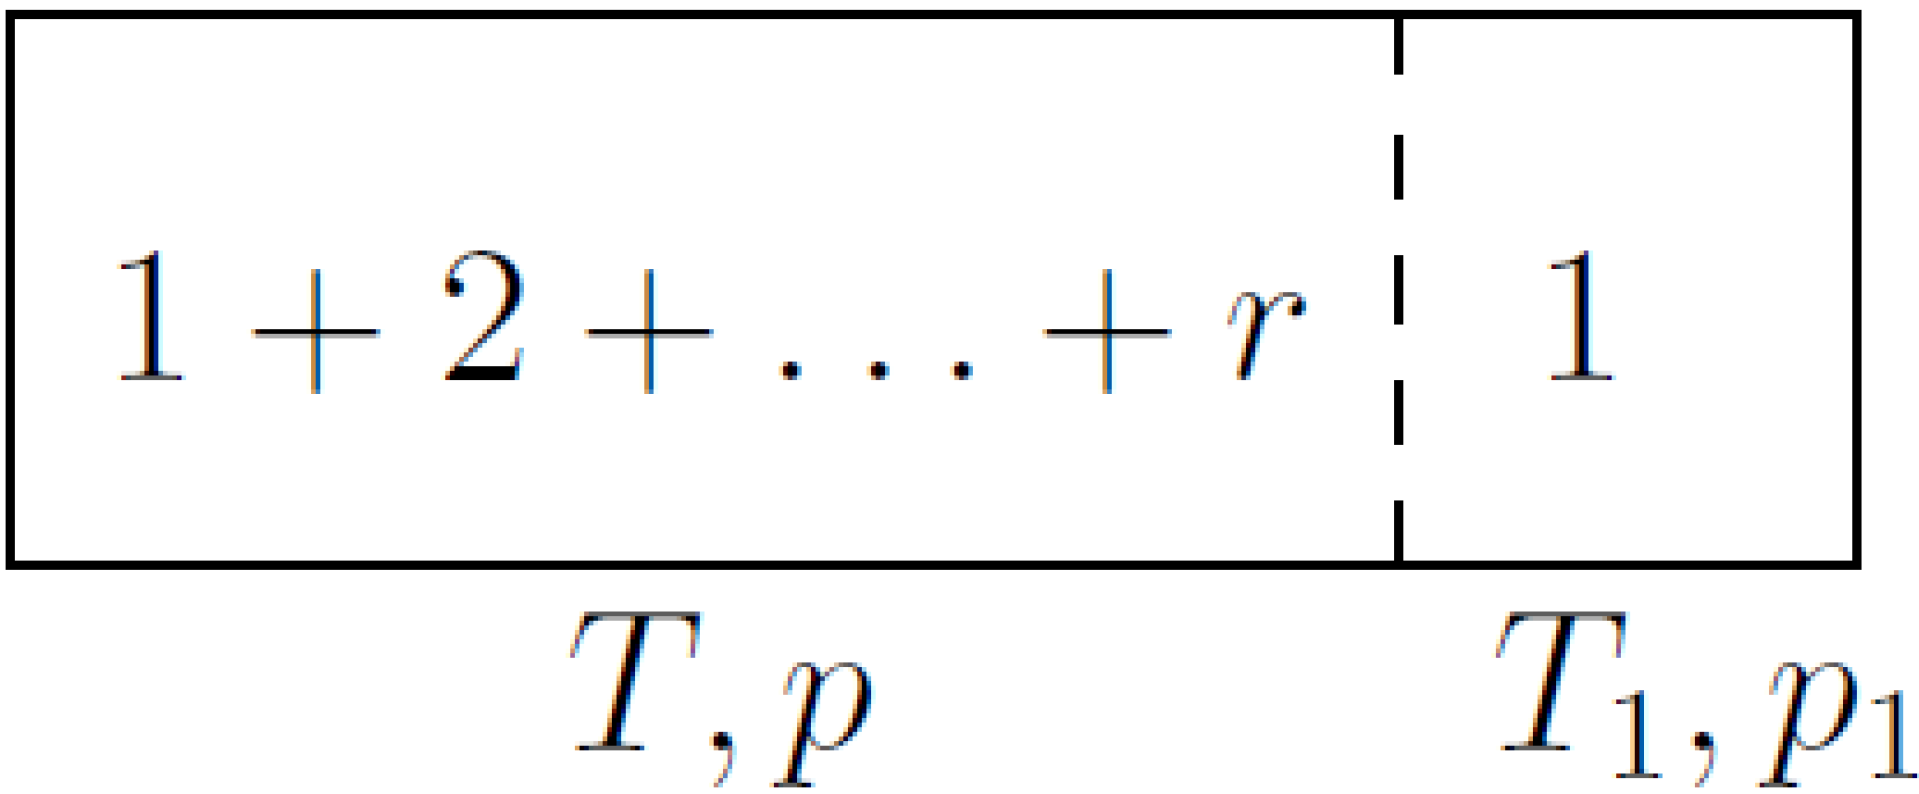
\includegraphics[width=\textwidth]{Bilder/Osmotischer_Druck.png}
\end{minipage}
austauschen lässt.
Gleichgewichtsbedingung: $T = T_1$ und $\mu_1 (T,p,c_1,\dots,c_r) = \mu_1^0 (T,p_1)$.
Wir nehmen an $c_i \ll c_1 \ \forall i = 2,\dots,r$ und $c_1 \approx 1$.
\begin{align*}
    \tilde{\mu}_1^0 (T,p) - \mu_1^0 (T,p_1) = R T \sum_{i=2}^r c_i
    \approx
    \mu_1^0 (T,p) - \mu_1^0 (T,p_1)
\end{align*}
Nach Linearisieren:
\begin{align*}
    \frac{\partial \mu_1^0}{\partial p} \Big|_T (p-p_1)
    = v_1 (p-p_1)
    = R T \sum_{i=2}^r c_i
\end{align*}
Für den osmotischen Druck $p-p_1$ folgt:
\begin{align*}
    p - p_1 = \frac{R T \sum_{i=2}^r c_i}{v_1}
\end{align*}

\subsubsection{Lösung eines idealen Gases}

\begin{minipage}{0.22\textwidth}
    Ein Gas ist gelöst in einer Flüssigkeit. Der Druck und die Temperatur sind fix.
\end{minipage} \hspace{5pt}
\begin{minipage}{0.25\textwidth}
    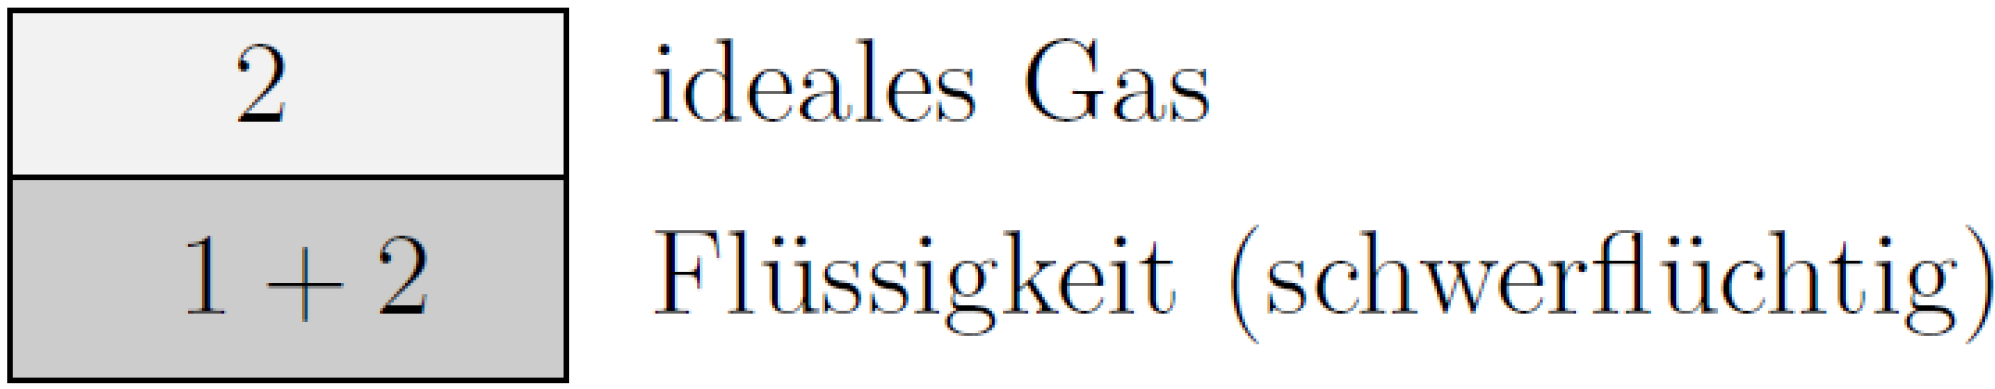
\includegraphics[width=\textwidth]{Bilder/Loesung_ideales_gas.png}
\end{minipage}

Für $\overline{\mu}_2^0$ dem chemischen Potential der reinen Gasphase und $\mu_2$
demjenigen der Mischung gilt:
\begin{align*}
    \mu_2 (T,p) = \overline{\mu}_2^0 (T,p) = \tilde{\mu}_2^0 (T,p) + R T \log(c_2)
    \\
    \frac{\partial \overline{\mu}_2^0}{\partial p} \Big|_T = \overline{v}_2
    \stackrel{\text{id. Gas}}{=} \frac{R T}{p}
    \hspace{10pt} , \hspace{10pt}
    \frac{\partial \tilde{\mu}_2^0}{\partial p} \Big|_T = \tilde{v}_2
\end{align*}
Hier sind $\overline{v}_2$ das Molvolumen des idealen Gases und $\tilde{v}_2$ die
Änderung des Lösungsvolumens bei der Lösung eines Mols des Gases. Unter der Annahme
$\tilde{v}_2 \ll \overline{v}_2$ gilt $\overline{v}_2 - \tilde{v}_2 \approx \overline{v}_2$
und aus $\overline{v}_2 \approx R T \frac{\partial}{\partial p} \log(c_2)$ erhalten
wir das \fat{Henry-Gesetz}.
\begin{align*}
    \frac{\partial \log(c_2)}{\partial p} \Big|_T = \frac{1}{p} = \frac{d \log(p)}{dp}
    \hspace{10pt} \Rightarrow \hspace{10pt}
    c_2 = \text{const} \cdot p
\end{align*}

\subsubsection{Konzentrationsverhältnisse in zwei nicht mischbaren Lösungsmitteln}

Betrachte zwei nicht mischbare Lösungsmittel $1$ und $1^\star$ und Substanzen
$2,\dots,r$ die gelöst sind in den Lösungsmitteln. Gleichgewichtsbedingung:
$\tilde{\mu}_i^0 (T,p) + R T \log(c_i) = \tilde{\mu}_i^{\star 0} (T,p) + R T \log(\overline{c}_i)$
wobei die linke Seite das chemische Potential in der Lösungs $1$ ist und die rechte
Seite dasjenige in der Lösung $1^\star$ ist. Es folgt die \fat{Nernst-Gleichung}:
\begin{align*}
    \frac{\overline{c}_i}{c_i} = e^{\frac{\tilde{\mu}_i^0 - \tilde{\mu}_i^{\star 0}}{R T}}
\end{align*}

\subsubsection{Phasengleichgewicht binärer Systeme}

\begin{figure}[h]
    \centering
    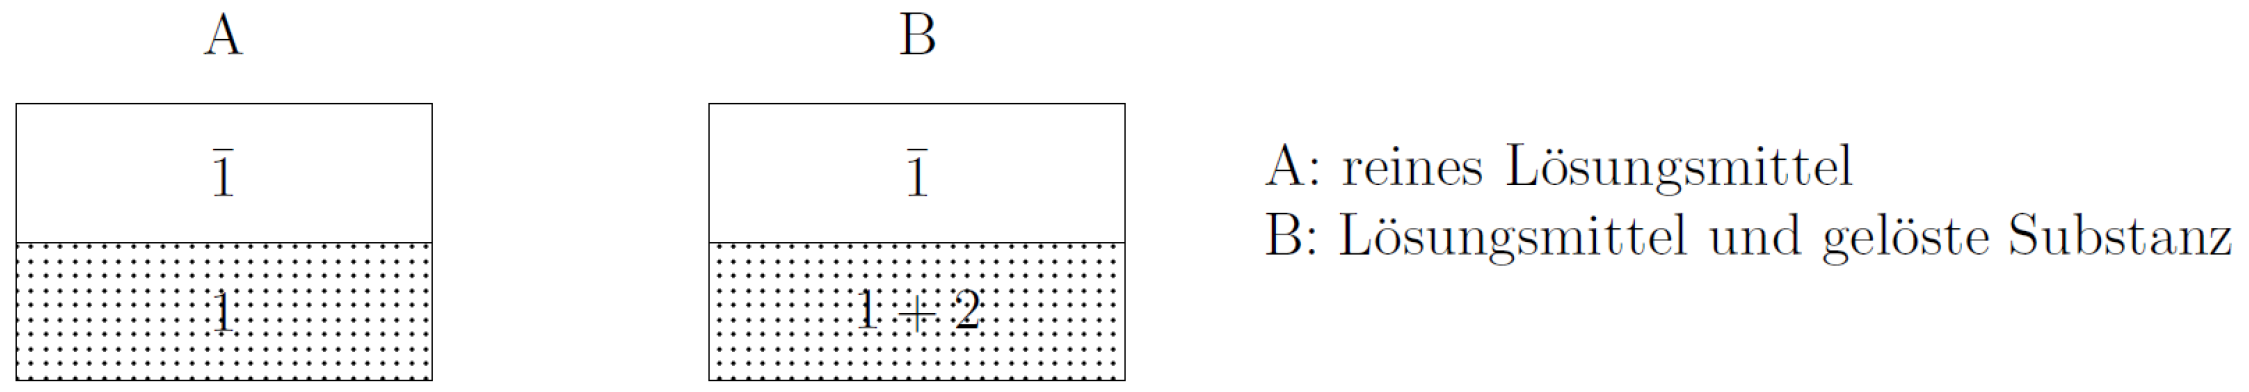
\includegraphics[width=0.48\textwidth]{Bilder/Phasengleichgewicht_binaere_Systeme.png}
\end{figure}

Gleichgewichtsbedingung: $\overline{\mu}_1^0 (T,p) = \mu_1 (T,p)$. Wobei
$\overline{\mu}_1^0 (T,p)$ das chemische Potential der ersten Substanz in Phase
$\overline{1}$ ist und $\mu_1 (T,p)$ das von der reinen Phase $1$ (A) respektive der
Lösung $1+2$ (B) bezeichnet. Nach Linearisierung:
\begin{align*}
    \overline{\mu}_1^0 (T^\ast,p^\ast) = \mu_1^0 (T,p) \hspace{10pt} (A)
    \hspace{10pt} , \hspace{10pt}
    \overline{\mu}_1^0 (T,p) = \mu_1^0 (T,p) - R T c_2 \hspace{10pt} (B)
\end{align*}
wobei $T^\ast$ und $p^\ast$ die Temperatur und der Druck sind wo der erste Stoff ohne
das Lösungsmittel im Gleichgewicht ist. Weiter gilt:
\begin{align*}
    \frac{\partial \mu_1^0}{\partial p} \Big|_T = v_1
    \hspace{10pt} , \hspace{10pt}
    \frac{\partial \mu_1^0}{\partial T} \Big|_p = - s_1
    \hspace{10pt} , \hspace{10pt}
    \frac{\partial \overline{\mu}_1^0}{\partial p} \Big|_T = \overline{v}_1
    \hspace{10pt} , \hspace{10pt}
    \frac{\partial \overline{\mu}_1^0}{\partial T} \Big|_p = - \overline{s}_1
\end{align*}
Mit $\Delta p = p - p^\ast$ und $\Delta T = T-T^\ast$ gilt:
\begin{align*}
    \mu_1^0 (T^\ast + \Delta T,p^\ast + \Delta p) &= \mu_1^0 (T^\ast,p^\ast) + v_1 \Delta p - s_1 \Delta T
    \\
    \overline{\mu}_1^0 (T^\ast + \Delta T,p^\ast + \Delta p) &= \overline{\mu}_1^0 (T^\ast,p^\ast) + \overline{v}_1 \Delta p - \overline{s}_1 \Delta T
    \\
    \Rightarrow \overline{\mu}_1^0 - \mu_1^0 &= (\overline{v}_1 - v_1) \Delta p - (\overline{s}_1 - s_1) \Delta T
    \\
    \Rightarrow - R T c_2 &= (\overline{v}_1 - v_1) \Delta p - (\overline{s}_1 - s_1) \Delta T
\end{align*}
Für $c_2 = 0$ erhalten wir die Clausius-Clepeyron Gleichung.
\begin{itemize}
    \item \underline{Dampfdruckniedrigung} ($\Delta T = 0$). Raoultsches Gesetz:
        \begin{align*}
            \Delta p = - \frac{R T c_2}{\overline{v}_1 - v_1}
        \end{align*}
    \item \underline{Siedepunktserhöhung / Gefrierpunktsniedrigung} ($\Delta p = 0$).
        \begin{align*}
            \Delta T = \frac{R T c_2}{\overline{s}_1 - s_1} = \frac{R T^2 c_2}{L_{1\overline{1}}}
        \end{align*}
        wobei $L_{1 \overline{1}}$ die Übergangswärme ist.
\end{itemize}

\subsection{Chemische Gleichgewichte}

Nun betrachten wir Reaktionen, bei denen sich die Stoffzahlen ändern können.
Seien $A_1,\dots,A_r$ die involvierten Stoffe die $s$ Reaktionen durchlaufen.
Es gilt:
\begin{align*}
    \sum_{i=1}^r \nu_i^k A_i
    \hspace{10pt} (k=1,\dots,s)
\end{align*}
mit $\nu_i^k \ \in \N$ den stöchiometrischen Koeffizienten

\begin{beispiel}
    Für $2 H_2 + O_2 \leftrightharpoons 2 H_2 O$ schreibt man
    $-2 H_2 - O_2 + 2 H_2 O = 0$ und somit $\nu = (-2,-1,2)$.
\end{beispiel}

Die Molzahlen $N_1,\dots,N_r$ können sich im materiell abgeschlossenen System
wie folgt verändern
\begin{align*}
    d N_i = \sum_{k=1}^s \nu_i^k d \lambda^k
    \hspace{10pt} \Rightarrow \hspace{10pt}
    N_i = N_i^0 + \sum_{k=1}^s \nu_i^k \lambda_i^k
\end{align*}
Hier ist $d \lambda^k$ der Grad bis zu dem die $k$-te Reaktion abgelaufen ist.
Falls $d \lambda^k = 1$ und $d \lambda^j = 0 \ \forall j \neq k$, erhalten
wir die Gleichgewichtsbedingung
\begin{align*}
    0 &= d G = \sum_{i=1}^r \frac{\partial G}{\partial N_i} d N_i
    = \vec{\nu} \cdot d \vec{N}
    = \sum_k \vec{\mu} \cdot \vec{\nu}^k d \lambda^k
    \\
    &\Rightarrow
    \sum_{i=1}^r \nu_i^k \mu_i = 0 \ \ \forall k = 1,\dots,s
\end{align*}

\begin{bemerkung}
    Es gilt:
    \begin{align*}
        G_i = N_i \mu_i = U_i - T S_i + p V_i
        \ \ \Rightarrow \ \
        \mu_i = u_i - T s_i + p v_i
    \end{align*}
    A priori können die Energie und die Entropie beliebig normiert sein.
    \begin{align*}
        u_i \mapsto u_i + a_i
        \hspace{10pt} , \hspace{10pt}
        s_i \mapsto s_i + b_i
        \hspace{10pt} \Rightarrow \hspace{10pt}
        \mu \mapsto \mu_i + a_i - b_i T =: \tilde{\mu}_i
    \end{align*}
    Die Normierungskonstanten müssen erfüllen:
    \begin{align*}
        \sum_{i=1}^r \nu_i^k (\mu_i + a_i - T b_i) = 0
        \hspace{10pt}
        k=1,\dots,s
    \end{align*}
\end{bemerkung}

\paragraph{Reaktionen in idealen Gasen}
Das chemische Potential der Komponenten im Gemisch:
\begin{align*}
    \mu_i (T,p,c_1,\dots,c_r) = \mu_i^0 (T,p) + R T \log(c_i)
\end{align*}
wobei $\mu_i^0(T,p)$ das chemische Potential der reinen Komponente bezeichnet.
Es folgt das \fat{Massenwirkungsgesetz}:
\begin{align*}
    \prod_{i=1}^r c_i^{\nu_i} =
    \exp \klammer{- \frac{1}{R T} \sum_i \nu_i \mu_i^0(T,p)}
    =: K(T,p)
\end{align*}
$K(T,p)$ hängt nur von $T$ und $p$ ab und bestimmt den Gleichgewichtszustand
$N_1,\dots,N_r$ auf der stöchiometrischen Geraden $N_i = N_i^0 + \lambda \nu_i$.

Wichtige Merkmale sind Volumenänderungen $\Delta V$ und Reaktionswärme $Q$.
Das Entfernen einer Wand bei festem $T$ und $p$ sind i.A. irreversibel. Nach
Einstellung des Gleichgewichts: $\Delta U = - p \Delta V + Q$. Mit
$H = p V + U$ folgt $Q = \Delta H$. Die Reaktion heisst endotherm, falls
$\Delta H > 0$ und exotherm, falls $\Delta H < 0$.

\subsubsection{Spezialfall: Ideale Gase}

Für ideale Gase sind innere Energie $U_i$ und Partialdrücke $p_i$ additiv.
\begin{align*}
    H(S,p,N_1,\dots,N_r) &= \sum_{i=1}^r H_i (S_i , p_i , N_i)
    \\
    H(T,p,N_1,\dots,N_r) &= \sum_{i=1}^r H_i(T,p_i,N_i) = \sum_{i=1}^r N_i h_i (T,p_i)
\end{align*}
Mit $h_i(T,p) = u_i(T) + p v_i(T,p) = u_i (T) + R T \equiv h_i(T)$.
\begin{align*}
    \Delta H &= \Delta \lambda \sum_{i=1}^r \nu_i h_i (T)
    \\
    \Delta V &= \Delta \lambda \sum_{i=1}^r \nu_i v_i (T,p)
        = \Delta \lambda \frac{R T}{p} \underbrace{\sum_{i=1}^r \nu_i}_{=: \nu}
\end{align*}
Hier ist $\nu$ die Anzahl der in der Reaktion gewonnenen/verlorenen Teilchen.
Für die $(T,p)$-Abhängigkeit des Gleichgewichts gilt wegen
\begin{align*}
    \frac{\partial \mu_i^0}{\partial p} \Big|_T = v_i
    \hspace{5pt} &, \hspace{5pt}
    \frac{\partial \mu_i^0}{\partial T} \Big|_p = - s_i
    \hspace{5pt} , \hspace{5pt}
    \frac{d h_i}{d T} = c_p^i (T)
\end{align*}
mit $c_p^i$ die isobare spezifische Wärme, dass
\begin{align*}
    \frac{\partial \log(K)}{\partial p} \Big|_T
    &= - \frac{1}{R T} \underbrace{\sum_{i=1}^r \nu_i v_i (T,p)}_{\Delta V}
    = - \frac{\nu}{p}
    \\
    \frac{\partial \log(K)}{\partial T} \Big|_p
    &= \frac{1}{R T^2} \sum_{i=1}^r \nu_i \underbrace{(\mu_i^0 + T s_i)}_{h_i = \Delta V}
    = \frac{\Delta H}{R T^2} = \frac{Q}{R T^2}
    \\
    \frac{\mathrm{d}}{\mathrm{d} T} \Delta H(T)
    &= \sum_{i=1}^r \nu_i c_p^i (T)
\end{align*}
Mit $\Delta V$ der Volumenänderung bei einmaligem Umsatz $\Delta \lambda = 1$ der
Reaktion. Für $\Delta V = 0,\nu=0$ ist $K$ unabhängig von $p$ und somit ist das
Gleichgewicht druckunabhängig. $\Delta H$ ist die Entropieänderung und Reaktionswärme
bei einmaligem Umsatz.



\section{Klassische Statistische Mechanik}

\setcounter{subsection}{-1}

Ein klassisches System wird in der klassischen statistischen Mechanik
beschrieben durch die Angabe eines endlichen 'Gefässes' $\Lambda \subseteq
\R^3$, des Phasenraums $\Gamma_N = \R^{6N}$, der Hamiltonfunktion $H$, und
eines Zustandes. Der Zustand ist hier das Wahrscheinlichkeitsmass
$d \mu(x) = \omega(x) dx$ auf dem Phasenraum $\Gamma_N$. Wir bezeichnen
$\omega$ manchmal als die "Dichte". Reine Zustände haben eine Dichte der
Form $\omega(x) = \delta(x-x_0)$ für ein $x_0 \in \Gamma$. Alle anderen
Zustände heissen gemischt.

Die Zeitevolution eines klassischen mechanischen Systems ist gegeben durch
den Hamilton'schen Fluss $x \mapsto \phi_t(x)$. Demnach ist die Zeitevolution
eines 'statistischen' Zustandes $\omega_t(x) = \omega(\phi_{-t}(x))$.
Es gilt: $D \phi_t = 1$.

\subsection{Gibbs Paradox}

Betrachte ein Gasgemisch. Mit semipermeablen Wänden lassen sich die Stoffe
trennen. Wir nennen diesen Prozess $p$. Die dabei aufgewendete Arbeit ist
\begin{align*}
    W = N R T \log(2) = -Q
    \hspace{10pt} , \hspace{10pt}
    W = n k_B T \log(2)
\end{align*}
mit $N$ der Anzahl Mol des Stoffes und $n$ die Anzahl der Teilchen des Stoffes.
Dieser Prozess ist reversibel. Betrachte den Spezialfall $n=2$. Hier könnte man
einen alternativen Prozess $\overline{p}$ benutzen um die zwei Teilchen zu trennen:
man kann eine Wand einschieben. Dieser Prozess kostet keine Arbeit. Nun gilt
aber: $W(p^{-1} \circ \overline{p}) = - 2 k_B T \log(2)$ und $p^{-1} \circ
\overline{p}$ ist zyklisch. Dies ist ein Wiederspruch zum 2. HS! Betrachte
das folgende Setup. Zwei Behälter mit einer Trennwand und zwei Stoffen mit je
einem Molekül sollen am Schluss gleich getrennt sein, wobei am Anfang die
Moleküle auf verschiedenen Seiten der Trennwand sind für die zwei Behälter.
Ein Agent Memory wird eingeführ der misst welcher der beiden Stoffe auf der
linken Seite des Behälters ist und diese Information speichert. Solange die
Behälter nicht identisch sind, wird immer wieder die Trennwand entfernt und
neu eingefügt. Diese Prozesse kosten keine Arbeit. Das Paradox wird nun damit
erklärt, dass es Arbeit kostet um ein Bit Speicher zu löchen/initialisieren.
Diese Arbeit beträgt mindestens $k_B T \log(2)$. Dies ist bekannt als das
Bennett-Landauer-Prinzip. Das löschen des Memory (zwei Bits) braucht
$W = 2 k_B T \log(2)$ Arbeit.

\subsection{Die mikrokaninische Gesamtheit}

\begin{definition}[Ensemble/Gesamtheit]
    Ein Ensemble (auch Gesamtheit) ist eine Menge gleichartiger präparierter
    Systeme von Teilchen im thermodynamischen Gleichgewicht.
    Es gibt drei verschiedene Ensembles: Das mikrokanonische, das kanonische
    und das grosskanonische. Beim mikrokanonischen sind Energie, Teilchenzahl
    und Volumen fixiert, beim kanonischen nur die Teilchenzahl und das Volumen
    und beim grosskanonischen nur noch das Volumen.
\end{definition}

\subsubsection{Die Ergodenhypothese}

\begin{definition}[Erwartungswert]
    Der Erwartungswert einer Observablen $f=f(x)$ zur Zeit $t$ für ein
    System, welches zur Zeit $t=0$ im Zustand $\omega$ ist, ist definiert
    als
    \begin{align*}
        \langle f \rangle_{\omega_t} := \int_{\Gamma_N} d x \ \omega_t(x) f(x)
        = \int_{\Gamma_N} dx \ \omega(x) f(\phi_t(x))
    \end{align*}
    Die letzte Gleichheit gilt, weil der Hamiltonsche Fluss volumenerhaltend ist.
    Gleichbedeutend: $D \phi_t = 1$.
\end{definition}

Der Wiederkehrsatz von Poincaré sagt, dass für volumenerhaltende Flüsse fast
alle Punkte $x_0 \in \Gamma_N$ Wiederkehrpunkte sind. Insbesondere konvergiert
$\langle f \rangle_{\omega_t}$ für $t \rightarrow \infty$ für die meisten
Zustände gar nicht.

\begin{definition}[Zeitmittelwert]
    Nach dem Ergodensatz von Birkhoff, existiert für jede Verteilung $\omega$
    der Zeitmittelwert:
    \begin{align*}
        \langle f \rangle_{\overline{\omega}} :=
        \limes{T \rightarrow \infty} \frac{1}{T} \int_0^T dt \ \langle f \rangle_{\omega_t}        
    \end{align*}
    Wir deuten diesen als Erwartungswert im thermodynamischen Gleichgewicht.
\end{definition}

\begin{definition}[Wahrscheinlichkeitsdichte]
    Die Wahrscheinlichkeitsdichte ist die zeitgemittelte Dichte $\omega_t$:
    \begin{align*}
        \overline{\omega} := \limes{T \rightarrow \infty} \frac{1}{T} \int_0^T dt \ \omega_t
    \end{align*}
\end{definition}

\begin{definition}[Mikrokanonische Gesamtheit]
    Die mikrokaninische Gesamtheit bei Energie $E$ ist der Zustand
    \begin{align*}
        \omega_E(x) := \frac{1}{\Sigma (E)} \delta(H(x)-E)
    \end{align*}
    und die zugehörige Zustandssumme ist:
    \begin{align*}
        \Sigma(E) := \int_{\Gamma_N} dx \ \delta(H(x)-E)
    \end{align*}
    Weil $H$ invariant ist unter dem Gluss $\phi_t$ ist es auch das Wahrscheinlichkeitsmass
    $d \mu_E = \omega_E (x) dx$ invariant, genau so wie die Energiefläche
    $\Gamma_N (E) = \geschwungeneklammer{x \in \Gamma_N \ | \ H(x) = E}$.
\end{definition}

\begin{bemerkung}
    \begin{enumerate}[1)]
        \item $\omega_E$ hat nur Support auf $\Gamma_N (E)$
        \item $\omega_{E,t} = \omega_{E,0} (\phi_{-t}(x)) = \omega_E (x)$
            da $\omega_E$ invariant ist unter $\phi_t$.
    \end{enumerate}
\end{bemerkung}

\begin{bemerkung}
    $\omega_E$ ist diejenige Verteilung auf $\Gamma_N (E)$, welche die
    Informationstheoretische Entropie $S(\omega)$ maximiert.
    \begin{align*}
        S(\omega) = - k_B \int_{\Gamma_N} dx \ \omega(x) \log \klammer{\omega(x) h^{3N}}
    \end{align*}
\end{bemerkung}

\paragraph{Ergodenhypothese}
Fast alle Bahnen der Energie $E$ kommen jedem Punkt in $\Gamma_N (E)$ immer
wieder beliebig nahe und zwar gleichmässig oft. $\Leftrightarrow$ Das einzige
unter $\phi_t$ invariante Wahrscheinlichkeitsmass auf $\Gamma_N (E)$ ist
die mikrokaninische Gesamtheit.

\vspace{1\baselineskip}

Nach der Ergodenhypothese gilt für jeden Zustand der Form
$\omega(x) = \tilde{\omega}(x) \delta(H(x)-E)$ für feste Energie $E$:
$\overline{\omega} = \omega_E$. Die zeitgemittelte Verteilung ist also die
mikrokanonische. Dies impliziert für jede Funktion $f$ auf dem Phasenraum
$\Gamma_N$, dass ihr Zeitmittel gleich dem Ensemblemittel ist:
$\langle f \rangle_{\overline{\omega}} = \langle f \rangle_{\omega_E}$.

\begin{bemerkung}
    Für allgemeine Zustände
    \begin{align*}
        \omega(x) dx = \int dE \ \klammer{\tilde{\omega}(x) \delta(H(x) - E) dx}
    \end{align*}
    lässt sich der Zeitmittelwert als Mittelwert über das Ensemble beschreiben.
    \begin{align*}
        \langle f \rangle_{\overline{\omega}} = \int d E \ W_E \int_{\Gamma_N} dx \ \omega_E (x) f(x)
    \end{align*}
    wobei
    \begin{align*}
        W_E = \int dx \ \tilde{\omega}(x) \delta(H(x)-E)
    \end{align*}
    somit sind die Erwartungswerte von Observablen im thermodynamischen
    Gleichgewicht alleine durch die Energieverteilung $W_E$ bestimmt.
\end{bemerkung}

\subsubsection{Das Gibbs'sche Variationsprinzip}

\begin{definition}[Informationstheoretische Entropie]
    $x \in \Omega$ abzählbar. $p$: Wahrscheinlichkeitsverteilung auf $\Omega$
    sodass $\sum_{x \in \Omega} p(x) = 1$.
    \begin{align*}
        S_{IT} = - \sum_{x \in \Omega} p(x) \cdot \log_2 (p(x))
    \end{align*}
    Hierbei haben wir $\omega(x)$ diskretisiert zu $p(x)$:
    \begin{align*}
        p(x) = \int_{\sigma(x)} \omega \ dx \approx \omega(x) h^{3N}
    \end{align*}
    Wobei $\sigma \in \Gamma_N$ von Volumen $h^{3N}$ ist.
\end{definition}

\begin{definition}[Statistische-Mechanik Entropie]
    Wir definieren die Entropie einer Wahrscheinlichkeitsverteilung $\omega$
    auf $\Gamma_N$ als
    \begin{align*}
        S_{SM}(\omega) := - k_B \int_{\Gamma_N} dx \ \omega(x) \log \klammer{\omega(x) h^{3N}}
    \end{align*}
    wobei $h>0$ eine Konstate mit der Dimension einer Wirkung ist.
\end{definition}

\begin{bemerkung}
    \begin{align*}
        S_{SM}(\omega) = - k_B \sum_x \underbrace{h^{3N} \omega(x)}_{= p(x)} \ln \klammer{\omega(x) h^{3N}}
        = - k_B \ln(2) S_{IT}(p)
    \end{align*}
\end{bemerkung}

\begin{bemerkung}
    Die so definierte Entropie $S(\omega)$ lässt sich interpretieren als
    Mass für die fehlende 'Information', die nötig wäre um den reinen Zustand
    eines Systems bis zur Präzision $h^{3N}$ zu bestimmen. Wenn man $n$ Stichproben
    $x_1,\dots,x_n$ gemäss Wahrscheinlichkeitsverteilung $\omega(x)$ nimmt, so
    ist die Anzahl Möglichkeiten die verschiedenen Stichproben aus den
    verschiedenen Zellen zu ziehen $\sim e^{n k_B^{-1} S(\omega)}$ und die
    Anzahl Ja/Nein-Fragen, die nötig wären um herauszufinden in welchem
    Zustand die $n$ Kopien des Systems sind, ist $\sim \frac{n}{K_B \log(2)}
    S(\omega)$.
\end{bemerkung}

\begin{lemma}[Eigenschaften der Entropie]


    \begin{enumerate}[(i)]
        \item Die Entropie ist strikt konkav: Für $\omega = \lambda \omega_1
            + (1-\lambda) \omega_2$, $0 \leq \lambda \leq 1$, gilt:
            \begin{align*}
                S(\omega) \geq \lambda S(\omega_1) + (1-\lambda) S(\omega_2)
            \end{align*}
            mit Gleichheit nur für $\lambda=0,1$ oder $\omega_1 = \omega_2$.
        \item Trennungssatz: Sei $\omega$ ein Zustand auf $\Gamma_N = \Gamma_{N_1}
            \times \Gamma_2$ mit $N=N_1+N_2$. Die Marginalverteilungen seien
            \begin{align*}
                \omega_1(x_1) = \int_{\Gamma_{N_2}} dx_2 \ \omega(x_1,x_2)
                \hspace{5pt} , \hspace{5pt}
                \omega_2(x_2) = \int_{\Gamma_{N_1}} dx_1 \ \omega(x_1,x_2)
            \end{align*}
            Diese sind Zustände auf $\Gamma_{N_1}$ respektive $\Gamma_{N_2}$.
            Es gilt: $S(\omega) \leq S(\omega_1) + S(\omega_2)$ mit
            Gleichheit genau dann, wenn die Systeme unkorreliert sind, d.h.
            falls $\omega(x_1,x_2) = \omega_1(x_1) = \omega_2 (x_2)$
        \item Die Entropie bleibt unter der Hamiltonschen Dynamik erhalten:
            $S(\omega_t) = S(\omega)$, wobei $\omega_t(x) = \omega(\phi_{-t}(x))$
            und $\phi_t$ der Hamiltonsche Fluss ist.
        \item Definiere den zeitgemittelten Zustand auf dem Zeitintervall $[0,T]$
            als
            \begin{align*}
                \overline{\omega}_T := \frac{1}{T} \int_0^T dt \ \omega_t
            \end{align*}
            Die Entropie dieser Zustände nimmt monoton mit $T$ zu:
            \begin{align*}
                S(\overline{\omega}_{nT}) \geq S(\overline{\omega}_T)
            \end{align*}
            für $T>0$ und $n=1,2,\dots$ Das heisst: die Unsicherheit über den
            eigentlichen Zustand nimmt zu, wenn $T$ grösser wird.
    \end{enumerate}
\end{lemma}

\paragraph{Gibbs'sches Variationsprinzip}
Unter allen Zuständen zu festen $N,E$ hat der Gleichgewichtszustand die
maximale Entropie.

\begin{lemma}[Maximierer der Entropie]
    Sei $\Omega \subset \Gamma_N$ eine Teilmenge des Phasenraums mit
    endlichem Volumen $0<\abs{\Omega}<\infty$ und $\omega$ eine Wahrscheinlichkeitsverteilung
    mit $\supp(\omega) \subset \Omega$. Unter all diesen Verteilungen
    maximiert die Gleichverteilung $\omega_u \equiv \abs{\Omega}^{-1}$ die
    Entropie.
\end{lemma}

\begin{theorem}[Mikrokanonische Gemamtheit und maximale Entropie]
    Für feste Energie $E$ und Teilchenzahl $N$ maximiert die mikrokanonische
    Gesamtheit die Entropie.
\end{theorem}

\begin{bemerkung}
    \begin{align*}
        \omega_E (x) h^{3N} &= p(x) = \frac{h^{3N}}{\Sigma(E,V,N)}
        \\
        S_{SM}(\omega_E) &= - k_B \int_{\Gamma_N} dx \ \omega_E (x) \log \klammer{\frac{h^{3N}}{\Sigma (E,V,N)}}
        \\
        &= k_B \log \klammer{\frac{\Sigma(E,V,N)}{h^{3N}}}
    \end{align*}
\end{bemerkung}

\begin{beispiel}[1-atomiges ideales Gas]
    Die Entropie des GGW Zst. ist
    \begin{align*}
        S(E,V,N) &= k_B \log \klammer{\frac{\Sigma(E,V,N)}{h^{3N}}}
        \\
        \Sigma(E,V,N) &= \int_{\Gamma_N} dx \ \delta(H(x) - E)
    \end{align*}
    Konkret gilt:
    \begin{align*}
        \Sigma(E,V,N) &=
        \int_{\Gamma_N} d^{3N} q \ d^{3N} p \ \delta (E - H(x))
        \\
        &= \int_{\Gamma_N} d^{3N} q \ d^{3N} p \ \frac{d}{dE} \theta(E - H(x))
        \\
        &= \frac{d}{dE} \int_{\Lambda^N} d^{3N} q \ \int_{\geschwungeneklammer{H(q,p) \leq E}} d^{3N} p
        \\
        &= \frac{d}{dE} V^N A_{3N} \klammer{2 m E}^{\frac{3 N}{2}}
        \equiv \frac{d}{dE} \phi(E)
        \\
        \phi(E) &:= \int_{\Gamma_N} dx \ \theta(E - H(x)) 
        \\
        A_d &= \frac{\pi^{d/2}}{\Gamma \klammer{\frac{d}{2} + 1}}
        \hspace{10pt} , \hspace{10pt} \Gamma(k+1) = k! \approx k^k e^{-k}
        \\
        S_{SM} &= k_B \klammer{\frac{3N}{2} + N \log \klammer{\klammer{\frac{4 \pi m E}{3 N}}^{3/2} \frac{1}{h^3}} + \log \klammer{\frac{3N}{2E}}}
    \end{align*}
Der letzte Term ist vernachlässigbar für grosse $N$.
\end{beispiel}

\subsubsection{Der Gleichverteilungssatz}

Wir betrachten ein Hamiltonsches System mit $f$ Freiheitsgraden und
arbeiten in den unabhängigen Koordinaten $(x_1,\dots,x_{2f}) =
(q_1,p_1,\dots,q_f,p_f)$. Der Hamiltonian sei $H = H(x)$.

\begin{theorem}[Gleichverteilungssatz]
    Sei $\langle \cdot \rangle$ der Mittelwert über die Wahrscheinlichkeitsverteilung
    im Gleichgewicht. Weiter sei $\Sigma(E)$ die mikrokanonische Zustandssumme
    und $\Phi(E)$ wie oben definiert. Es gilt
    \begin{align*}
        \left\langle x_i \frac{\partial H}{\partial x_j} \right\rangle
        \equiv \frac{1}{\Sigma(E)} \int_{\Gamma_N} dx \ \delta(H(x) - E) x_i \frac{\partial H}{\partial x_j}
        = \delta \eckigeklammer{\frac{d}{dE} \log(\Phi(E))}^{-1}
    \end{align*}
\end{theorem}

\begin{korollar}[Folgerung aus Gleichverteilungssatz]
    Mit der Definition der Entropie $S(E) = k_B \log(\Sigma(E)/h^{3N})$,
    und $\log(\Sigma(E)) \approx \log(\Phi(E))$ für grosse $N$, folgt
    \begin{align*}
        \left\langle x_i \frac{\partial H}{\partial x_j} \right\rangle
        = \delta_{ij} \eckigeklammer{\frac{1}{k_B} \frac{d}{dE} S(E)}^{-1}
        = \delta_{ij} k_B T
    \end{align*}
\end{korollar}

\begin{bemerkung}[Anwendung]
    Für $H = \sum_i \underbrace{\frac{1}{2 m} p_i^2}_{= K_i} + \sum_i \underbrace{c q_i^r}_{= V_i}$
    sei $x_i = q_k$ und $x_j = q_k$. Dann gilt:
    \begin{align*}
        \langle V_k \rangle = \frac{1}{r} \left\langle x_i \frac{\partial H}{\partial x_j} \right\rangle
        = \frac{1}{r} k_B T
        \hspace{10pt} , \hspace{10pt}
        \left\langle K_k \right\rangle = \frac{1}{2} k_B T
    \end{align*}
\end{bemerkung}

\paragraph{Beispiele}

\begin{enumerate}[(i)]
    \item \underline{1-atomiges Gas}: $V_i = 0$, $U = \frac{3}{2} N k_B T$,
        $c_v = \frac{\partial U}{\partial T} \Big|_V \frac{1}{N} = \frac{3}{2} k_B$
    \item \underline{2-atomiges Gas mit $d$ konstant}: $U = \frac{5 N}{2} k_B T N$,
        $c_V = \frac{5}{2} k_B$
    \item \underline{2-atomiges Gas mit Verbindung die um $d>0$ schwingt}:
        $V_{\text{Molekül}} = c \cdot \abs{x_{rel}}^2$,
        $x_{rel}$ in eine Dimension beschränkt,
        $c_V = \frac{5+1+1}{2} k_B = \frac{7}{2} k_B$, $x_{rel}$
    \item \underline{2 atomiges Gas mit Verbindung die um $d=0$ schwingt}:
        $V_{\text{Molekül}} = c \cdot \abs{x_{rel}}^2$,
        $x_{rel}$ in allen 3 Dimensionen:
        $V_{\text{Molekül}} = c \cdot \klammer{x_{rel,1}}^2 + c \klammer{x_{rel,2}}^2
        + c \klammer{x_{rel,3}}^2$,
        $c_V = \frac{3+2 \cdot 3}{2} k_B = \frac{9}{2} k_B$
\end{enumerate}
Der Übergang von schwingend zu steif ist unstetig und kann nur quantenmechanisch
erklärt werden. Den schwingenden Freiheitsgrad für grosse Schwingungsfrequenzen
muss man nicht berücksichtigen.

\subsection{Die kanonische Gesamtheit}

Betrachte zwei Systeme im thermischen Kontakt mit $V' \gg V$ und $N' \gg N$.
Die zwei Systeme können Wärme austauschen, doch ihre Volumen und Teilchenzahlen
bleiben konstant. Der Zustand des Gesamtsystems sei die mikrokanonische
Gesamtheit zur Energie $E$. Wir vernachlässigen die Wechselwirkung der beiden
Systeme und können desshalb annehmen: $H_0(x,x') = H(x) + H'(x')$.
Der Zustand des kleinen (ungestrichenen) Systems ist:
\begin{align*}
    \omega(x) &= \frac{1}{\Sigma_0 (E)} \int_{\Gamma_{N'}} dx' \delta(H(x) + H'(x) - E)
    \\
    &= \frac{1}{\Sigma_0 (E)} \Sigma'(E-H(x))
    = \frac{1}{\Sigma_0 (E)} e^{k_B^{-1} S'(E-H(x))}
\end{align*}
Taylorentwicklung von $S'$ nach $H(x)$:
\begin{align*}
    S'(E-H(x)) = \underbrace{S'(E)}_{\sim N'} - \underbrace{\frac{\partial S'}{\partial E}}_{=\frac{1}{T}}
    \underbrace{H(x)}_{\sim N} + \frac{1}{2} \underbrace{\underbrace{\frac{\partial^2 S'}{\partial E^2}}_{\sim \frac{1}{N'}}
    \underbrace{H(x)^2}_{\sim N^2}}_{\sim \frac{N}{N'} \cdot N} - \dots
\end{align*}
Im Limes $(E,V',N') \rightarrow \infty$ erhalten wir:
\begin{align*}
    \omega(x) &= \frac{1}{\Sigma_0(E)} e^{k_B^{-1} \klammer{S'(E) - \frac{1}{T} H(x)}}
    = \frac{1}{Z(\beta)} e^{-\beta H(x)}
    \\
    Z(\beta) &= \int_{\Gamma_N} e^{-\beta H(x)}
    = \int dE dx \ \delta(H(x)-E) e^{-\beta E}
    \\
    &= \int dE e^{-\beta E} \Sigma(E)
\end{align*}
$\omega(x)$ heisst kanonische Gesamtheit und $Z(\beta)$ ist die kanonische
Zustandssumme. Mit $\log(\omega(x)) = - \beta H(x) - \log(Z(\beta))$ folgt:
\begin{align*}
    S(\omega) = - k_B \int_{\Gamma_N} dx \ \omega(x) \log(\omega(x))
    = k_B \beta \langle H \rangle + k_B \log(Z(\beta))
\end{align*}
Für die freie Energie folgt:
\begin{align*}
    F(\beta) = U - T S \equiv \langle H \rangle - \frac{S}{k_B \beta}
    = - \frac{1}{\beta} \log(Z(\beta))
\end{align*}

\subsection{Die grosskanonische Gesamtheit}

Wir betrachten wieder zwei Systeme die nun aber im thermischen und materiellen
Gleichgewicht sind und somit sowohl Wärme als auch Teilchen austauschen. Es gilt:
$V' \gg V$, $H_0(x,x') = H(x) + H'(x')$ und $N_0 = N' + N$. Der Zustand des
kleineren Systems ist:
\begin{align*}
    \omega(N,x) &= \frac{1}{Z_0(\beta)} \int_{\Gamma_{N_0 - N}} dx' e^{-\beta H'(x')} e^{-\beta H(x)}
    \\
    &= \frac{e^{-\beta F'(\beta,N_0 -N)}}{Z_0(\beta)} e^{-\beta H(x)}
\end{align*}
Taylorentwicklung von $F'$ nach $N$ liefert:
\begin{align*}
    F'(\beta,N_0 - N) = F'(\beta,N_0) - \mu N + \mathcal{O} \klammer{\frac{1}{N_0}}
\end{align*}
Für den Zustand des kleinen Systems folgt:
\begin{align*}
    \omega(N,x) &= \frac{e^{-\beta \klammer{H(x) - \mu N}}}{\Xi (\beta,\mu)}
    \hspace{5pt} \text{mit} \\
    \Xi(\beta,\mu) &= \sum_{N=0}^\infty \int_{\Gamma_N} dx \ e^{-\beta(H(x)-\mu N)}
    = \sum_{N=0}^\infty z^N Z_N (\beta)
    \hspace{5pt} \text{mit} \hspace{5pt}
    z = e^{\beta \mu}
\end{align*}
$\omega(N,x)$ ist die grosskanonische Gesamtheit und $\Xi(\beta,\mu)$ ist
die Zustandssumme. $z$ wird auch als Fugazität bezeichnet. Wir definieren
das grosskanonische Potential $\Omega$ als
\begin{align*}
    \Omega(\beta,\mu) = U - T S - \mu N
    = - \frac{1}{\beta} \log \klammer{\Xi(\beta,\mu)}
\end{align*}

\subsection{Äquivalenz der Gesamtheiten}

\begin{figure}[H]
    \centering
    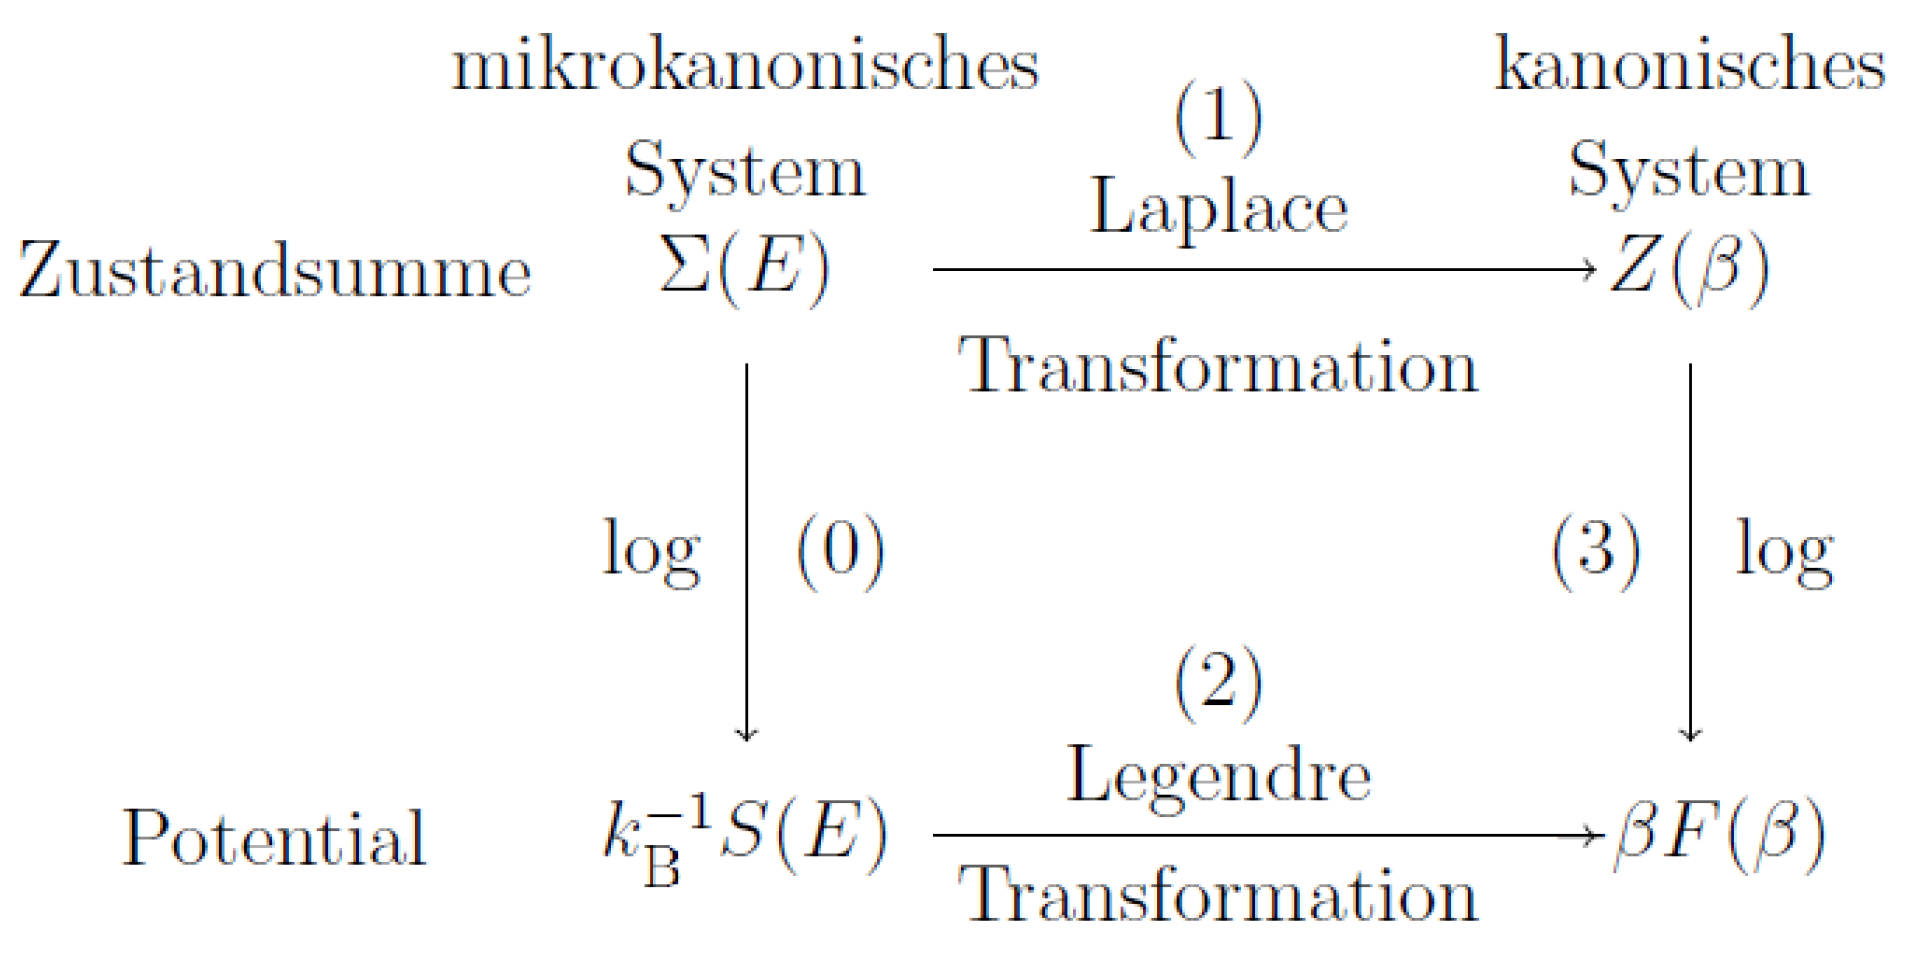
\includegraphics[width=0.3\textwidth]{Bilder/Aequivalenz_der_Gesamtheiten.png}
\end{figure}

Mittels Legendre Transformation erhalten wir:
\begin{align*}
    - \beta F_{mikro} (\beta) = - \beta \inf_S (U(S) - T S)
    = \sup_E (k_B^{-1} S_{mikro} (E) - \beta E)
\end{align*}
Wobei $S_{mikro}$ jene Entropie ist, welche aus dem mikrokanonischen Ensemble
hergeleitet wurde. Das Supremum wird angenommen für
\begin{align*}
    k_B^{-1} \frac{\partial S_{mikro}}{\partial E} = \beta
\end{align*}
Die kanonische Zustandssumme wird berechnet durch
\begin{align*}
    Z(\beta) &= \int dE \ d^{-\beta E} \Sigma(E)
    \equiv \int dE \ d^{g(E)}
    \\
    g(E) &= -\beta E + \log(\Sigma(E)) = - \beta E + k_B^{-1} S_{mikro} (E)
    \\
    g'(E) &= - \beta + k_B^{-1} \frac{\partial S_{mikro}}{\partial E}
    \\
    g''(E) &= k_B^{-1} \frac{\partial^2 S_{mikro}}{\partial E^2} = \mathcal{O}(1/N)
\end{align*}
Der grösste Beitrag zum Integral befindet sich bei der Energie $E=E_0$, wo
$g'(E_0) = 0$, d.h. wo
\begin{align*}
    k_B^{-1} \frac{\partial S_{mikro}}{\partial E} \Big|_{E_0} = \beta
\end{align*}
Mit der Näherung
\begin{align*}
    g(E) \approx g(E_0) + \frac{1}{2} g''(E_0) (E-E_0)^2
\end{align*}
wenden wir die Sattelpunkapproximation an und erhalten:
\begin{align*}
    Z(\beta) &\approx e^{-\beta E_0 + k_B^{-1} S_{mikro}(E_0)}
        \int dE \ e^{\frac{1}{2} g''(E_0)(E-E_0)^2}
    \\
    &= e^{-\beta F_{mikro}(\beta)} \underbrace{\mathcal{O} (\abs{g''(E_0)}^{-1/2})}_{= \mathcal{O}\klammer{N^{\frac{1}{2}}}}
\end{align*}
Somit ist
\begin{align*}
    F(\beta) \equiv - \beta^{-1} \log(Z(\beta)) = F_{mikro} (\beta) + \mathcal{O} \klammer{\log(N)}
\end{align*}

\subsection{Äquivalenz der Entropien}

Betrachte die informationstheoretische Entropie und die Statistische-Mechanik
Entropie. Wir betrachten nun den Grenzfall wo wir $\omega \rightarrow p$
diskretisieren.
\begin{align*}
    p(x) = \int_{\sigma(x)} \omega \ dx
    \approx \omega(x) \int_\sigma dx
    = \omega(x) h^{3N}
\end{align*}
wobei $\sigma \subset \Gamma_N$ von Volumen $h^{3N}$, d.h. $\int_\sigma dx = h^{3N}$.
$\sigma$ ist die kleinste Einheit die man betrachten kann. D.h. $\omega$ kann sich
darauf nicht ändern, bzw macht keinen Sinn. Damit folgt:
\begin{align*}
    S_{SM} (\omega) &= - k_B \sum_x h^{3N} \omega(x) \ln \klammer{\omega(x) h^{3N}}
    = - k_B \sum_x p(x) \ln \klammer{p(x)}
    \\
    &= k_B \ln(2) S_{IT} (p)
\end{align*}

Für ein 1-atomiges ideales Gas gilt: Bei einem Prozess bei dem $U_0 \rightarrow
U$ und $V_0 \rightarrow V$ ist
\begin{align*}
    S_{SM} &= k_B N \klammer{\frac{3}{2} + \log \klammer{\klammer{\frac{4 \pi m}{3}}^{3/2} \frac{1}{h^3}}}
        + k_B N \frac{3}{2} \log\klammer{\frac{E}{N}}
        \\ &\hspace{10pt}+ k_B N \log(V)
    \\
    \Delta S_{SM} &= k_B N \frac{3}{2} \log \klammer{\frac{U}{U_0}} + k_B N
        \log \klammer{\frac{V}{V_0}}
    \\
    \Delta S_{p} &= n \klammer{\int_{T_0}^T c_V \frac{dT}{T} + \int_{V_0}^V R \frac{dV}{V}}
    \\
    &= n c_v \log \klammer{\frac{U}{U_0}} + n R \log\klammer{\frac{V}{V_0}}
    \\
    \Rightarrow \hspace{5pt}
    R &= k_B \frac{N}{n} = k_B N_A
    \\
    c_v &= k_B \frac{N}{n} \frac{3}{2} = \frac{3}{2} R
\end{align*}
Wenn wir den Fall betrachten wo wir zwei Behälter mit jeweils $N$ Atomen und
Volumen $V$ zu einem Behälter mit $2N$ Teilchen und Volumen $2V$ zusammenführen
erhalten wir
\begin{align*}
    \Delta S_{p} &= 2N k_B \log(2N) - 2 N k_B \log(N) = 2N k_B \log(2)
    \\
    \Delta S_{SM} &= k_B 2N \log(2V) - 2 k_B N \log(V) = 2N k_B \log(2)
\end{align*}
Wir sehen, dass die SM Entropie derjenigen Entropie entspricht, wenn wir
annehmen, dass jedes Atom unterscheidbar ist.

Der einzige Term in der SM Entropie welcher nicht extensiv ist, ist $k_B N
\log(V)$. Wir nennen diesen Teil auch die Mischentropie. Falls wir annehmen,
dass die Teilchen ununterscheidbar sind, verschwindet dieser Term.


\subsubsection{Beweis der Äquivalenz}

Die Differenz der phenomenologischen Entropie wird durch einen Prozess $p$
beschrieben der ein System vom Zustand $\sigma_1$ in den Zustand $\sigma_2$
überführt: $\Delta S^p (p)$. Die Entropie der statistischen Mechanik nimmt
eine Wahrscheinlichkeitsverteilung $\omega$ als Argument: $S^{SM} (\omega)$.
Wir können mittels Gibbs'schem Variationsprinzip von $\sigma$ auf $\omega
= \omega(\sigma)$. Hierbei ist gemeint, dass $s^{SM}(\omega)$ maximiert wird
unter der Randbedingung $\sigma$. Wir haben bereits festgestellt, dass nur
Entropie Differenzen relevant sind. Wir wollen also zeigen, dass
\begin{align*}
    \Delta S^p (\sigma_1 \rightarrow \sigma_2) =
    S^{SM} (\omega(\sigma_2)) - S^{SM} (\omega(\sigma_1)).
\end{align*}
Wir bemerken ausserdem, dass der Referenzpunkt $S^{SM}(\omega_0) = 0$
von der Wahl von $h$ abhängt.
\begin{align*}
    \overline{S}^{SM} (\omega) &=
    - k_B \int dx \ \omega(x) \log \klammer{\omega(x) \overline{h}^{3N}}
    \\
    &= - k_B \int dx \ \omega(x) \log \klammer{\omega(x) h^{3N}}
    \\ &\hspace{20pt} - k_B \int dx \ \omega(x) \log \klammer{\klammer{\frac{\overline{h}}{h}}^{3N}}
    \\
    &= S^{SM} (\omega) - k_B 3N \klammer{\log(\overline{h}) - \log(h)}
\end{align*}
Weiter kann bewiesen werden, dass $S^{SM} (\omega)$ erhalten ist unter einem
Hamiltonischen Fluss $\phi_t$: $S^{SM} (\omega) = S^{SM} (\omega_t)$. Ausserdem
gelten die folgenden Eigenschaften:
\begin{enumerate}[(i)]
    \item $S^{SM}$ ist konkav mit WSK $p_0$ im Zst $\omega_0$ und mit Wsk
        $p_1$ im Zst $\omega_1$: $S^{SM} (p_0 \omega_0 + p_1 \omega_1) \geq
        p_0 S^{SM} (\omega_0) + p_1 S^{SM} (\omega_1)$.
    \item $S^{SM}$ ist additiv für unabhängige Systeme:
        $S^{SM} (\omega_A \times \omega_B) = S^{SM} (\omega_A) + S^{SM} (\omega_B)$
\end{enumerate}

Betrachte ein System mit Volumen $V$ und $N$ Teilchen welche durch eine Wand
in der linken Hälfte der Box gehalten werden. Betrachte nun den Prozess bei
dem die Wand entfernt wird. Die Entropie differenz ist dann gegeben als
\begin{align*}
    \Delta S^{IT} &= S^{IT}(\omega') - S^{IT}(\omega)
    \\
    &= \log_2 \klammer{V^N \int_{\geschwungeneklammer{H(p) = E}}}
        - \log_2 \klammer{\klammer{\frac{V}{2}}^N \int_{\geschwungeneklammer{H(p) = E}}}
    \\
    &= - \log_2 \klammer{\klammer{\frac{1}{2}}^N} = N 
\end{align*}
Hier ist $\omega$ die Wsk.verteilung vor dem Entfernen der Wand und $\omega'$
die Wsk.verteilung nach dem Entfernen der Wand. Allgemeiner gilt das folgende

\begin{theorem}
    Für jeden adiabatischen Prozess $\omega \rightarrow \omega'$ gilt immer
    \begin{align*}
        S^{SM} (\omega') \geq S^{SM} (\omega)
    \end{align*}
\end{theorem}

Im folgenden betrachten wir ein System wie oben mit $N=1$. D.h. wir sind im
gleichen Setup wie beim Gibbs'schen Paradox. Wir wählen den Referenzpunkt
der Entropie so, dass die Entropie der Systeme $M0$ und $M1$ bei denen man weiss
ob sich das Teilchen links oder rechts der Wand befindet Entropie $0$ hat. Nach
obiger Information über $\Delta S^{IT}$ folgt, dass das System $M?$ bei dem das
Teilchen mit $50 \%$-iger Wsk links oder rechts von der Wand ist, die Entropie
$1$ ist. Wir erinnern uns an die Betrachtung beim Gibbs'schen Paradox und stellen
fest, dass die Arbeit die für die Initialisierung $r$ benötigt wird um das System
$M?$ in entweder $M0$ oder $M1$ überzuführen gerade $W(r) = k_B T \log(2)$ ist.
Somit folgt für die Entropieänderung bei der Messung, dass
\begin{align*}
    \Delta S_M^p (r) = \frac{\Delta Q}{T} = - \frac{W}{T} = - k_b \log(2)
\end{align*}
Sei $K$ ein System auf dem ein reversibler Prozess $p$ das System vom
Zustand $\sigma_1$ in den Zustand $\sigma_2$ überführt. Die Entropieänderung
bei diesem Prozess ist gegeben als
\begin{align*}
    \Delta S_K^p (p) = \frac{\Delta Q_K (p)}{T} = S^p (\sigma_2) - S^p (\sigma_1)
\end{align*}
Betrachte nun das
System $K$, gekoppelt an ein Wärmereservoir $R$ bei Temperatur $T$, welches
wiederum an $\lambda$ viele Memorysysteme $M$ gekoppelt ist, was wir als
$M^\lambda$ schreiben. Ein Memorysystem ist ein Bit. Wir betrachten nun den
Prozess $r^\lambda \circ p$ der den Prozess $p$ ausführt und das Memorysystem
$M^\lambda$ resettet. Als $\lambda$ wählen wir nun
\begin{align*}
    \lambda = \frac{\Delta S_K^p}{k_B \ln(2)}
\end{align*}
Nun folgt:
\begin{align*}
    \Delta Q_R (p)
    &= - \Delta Q_K (p)
    = - T \Delta S_K^p (p)
    = - T \lambda k_B \ln(2)
    \\
    &= - \lambda T k_B \ln(2)
    = \lambda \Delta Q_M (r)
    = \Delta Q_{M^\lambda} (r^\lambda)
    \\
    &= - \Delta Q_R (r^\lambda)
\end{align*}
Somit folgt:
\begin{align*}
    \Delta Q_R (r^\lambda \circ p) = 0
\end{align*}
Da es sich um einen adiabatischen Prozess handelt, muss gelten
$\Delta S_{KRM}^{IT} (r^\lambda \circ p) \geq 0$. Daraus folgt:
\begin{align*}
    S_K^{IT} (\omega(\sigma_2)) + S_{M^\lambda} (M0^\lambda) + S_R
    &\geq
    S_K^{IT} (\omega(\sigma_1)) + S_{M^\lambda} (M?^\lambda) + S_R
    \\
    S_K^{IT} (\omega(\sigma_2)) - S_K^{IT} (\omega(\sigma_1))
    &\geq
    \lambda \klammer{S_{M}^{IT} (M?) - S_{M}^{IT} (M0)} = \lambda
    \\
    \Delta S_K^{IT}
    &\geq \frac{\Delta S_K^p}{k_B \ln(2)}
\end{align*}
Da der Prozess reversibel ist, gilt Gleichheit. Also folgt:
\begin{align*}
    \Delta S_K^p = k_B \log(2) \Delta S_K^{IT}
\end{align*}
\qed


\end{document}